\documentclass{book}
\title{A Computational Tour of Number Theory}
\author{Hao Chen \and R. Andrew Ohana \and Bharathwaj Palvannan
\and Travis Scholl
\and Simon Spicer \and William Stein \and
\and Yannick Van Huele}

\usepackage{macros}
\usepackage{hyperref}

\begin{document}
\maketitle
\tableofcontents

\chapter{Introduction: tour of the main objects}
In this book, we will explore several important central problems and
objects of number theory, and for each to explain how---in practice
(not just theory)---to {\em compute} with them.    Books,
papers, and web sites such as Wikipedia and Mathoverflow often
give excellent descriptions
of mathematical objects, algorithms, data, conjectures, and theorems.
However, they rarely give concrete instructions
so that you can manipulate them on a computer, with enough theoretical
discussion so that you understand the limitations and capabilities of
your tools.  That is the mission of the book you are looking at.


\section{Prime Numbers}

The prime numbers $2,3,5,7,11,\ldots, $ have fascinated
mathematicians for thousands of years.  Euclid proved there
are infinitely many: if $p_1,\ldots, p_n$ are primes,
then $p_1\cdots p_n + 1$ is an integer divisible by some
prime $p$ that isn't equal to any $p_i$.

Let's compute the primes up to 100:
\begin{lstlisting}
sage: prime_range(100)
[2, 3, 5, 7, 11, 13, 17, 19, 23, 29, 31, 37, 41, 43, 47, 53, 59, 61, 67, 71,
 73, 79, 83, 89, 97]
\end{lstlisting}
And draw a plot of the function $\pi(x)$ that counts the number of primes
up to $x$ for $x<100$.
\begin{center}
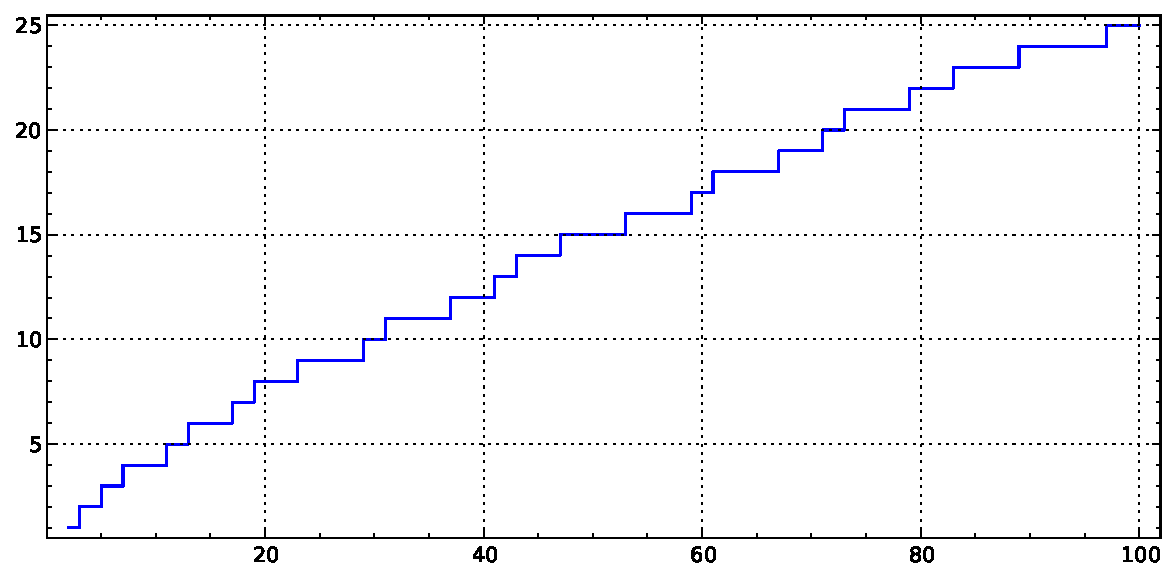
\includegraphics[width=.7\textwidth]{pics/prime_pi-2-100.pdf}
\end{center}

The {\em Prime Number Theorem}, which was proved over a century ago, asserts
that $\pi(x) \sim x/\log(x)$:

\begin{lstlisting}
@interact
def f(B=[10^n for n in [2..9]]):
    show(plot(lambda x: prime_pi(x)/(x/log(x)), (x,2,B))
       + line([(0,1),(B,1)],color='red'))
\end{lstlisting}

\begin{center}
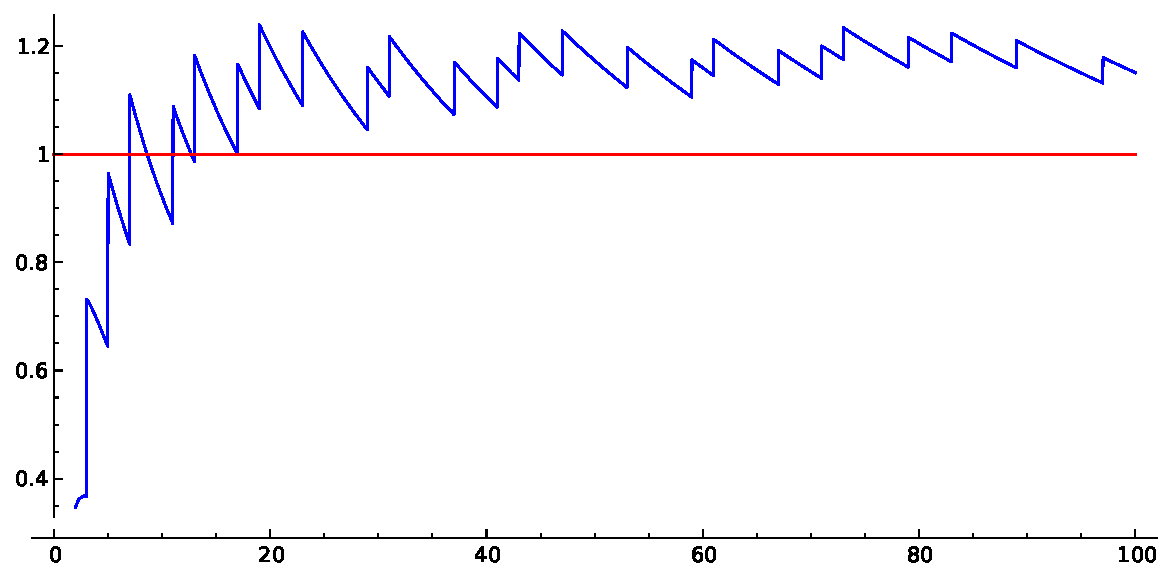
\includegraphics[width=.3\textwidth]{pics/pnt100.pdf}
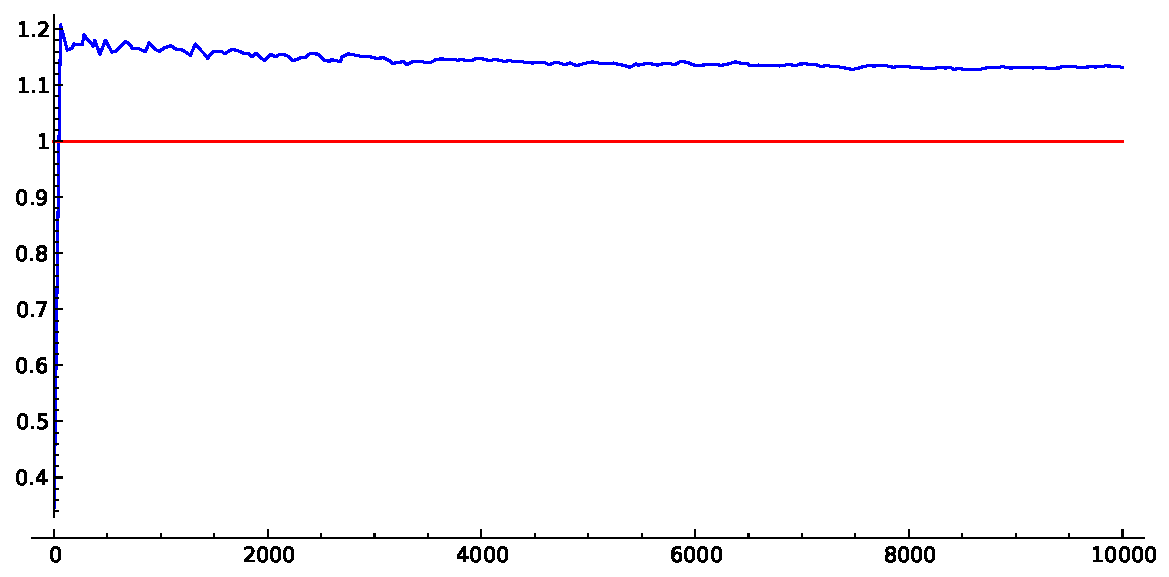
\includegraphics[width=.3\textwidth]{pics/pnt10000.pdf}
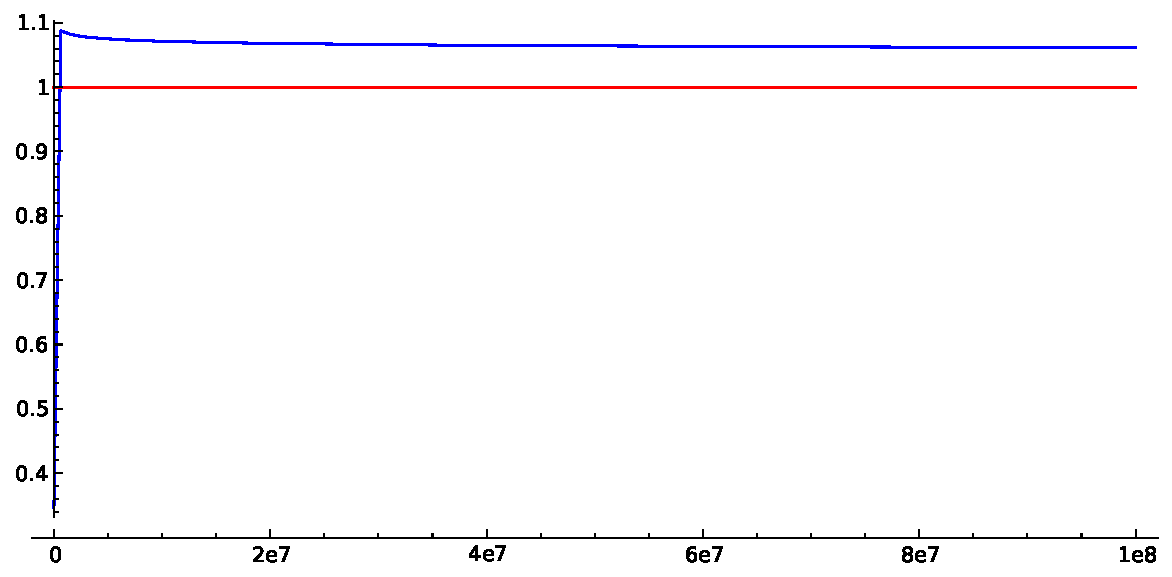
\includegraphics[width=.3\textwidth]{pics/pnt100000000.pdf}
\end{center}

The {\em Riemann Hypothesis}, which remains completely unsolved today,
asserts that for all $x\geq 2.01$,
$$
 |\pi(x) - \Li(x)| \leq \sqrt{x}\cdot \log(x),
$$
where
$$
 \Li(x) = \int_{2}^x \frac{dt}{\log(t)}
$$

In the range of the following plots, $\pi(x) - \Li(x)$ is
much smaller than $\sqrt{x}\log(x)$.
\begin{lstlisting}
@interact
def f(B=[10^n for n in [2..9]]):
    print "sqrt(B)*log(B) = ", round(sqrt(B)*log(B))
    show(plot(lambda x: prime_pi(x) - Li(x), (x,2,B)))
\end{lstlisting}
\begin{center}
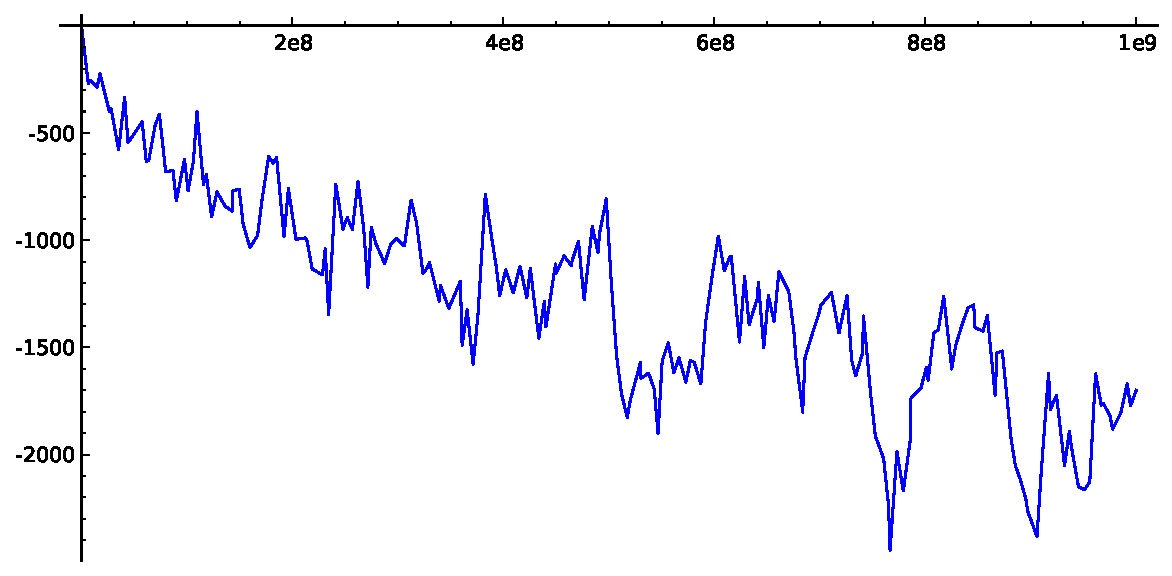
\includegraphics[width=.7\textwidth]{pics/pi_minus_li-1e9.pdf}
\end{center}
Up to $10^9$ we have $|\pi(x)-\Li(x)|$ is much
smaller than $\sqrt{10^9}\cdot \log(10^9) \sim  \num{655327}$.

\hw{Andrew and Bharath}{Can we prove anything toward $\sqrt{x}\cdot \log(x)$?}

% Basic calculus bound by Bharath
One can follow a naive approach and use basic calculus.
One sees easily that $\pi(x) \leq x$. Similarly, If $x \geq 2$, then $\log(x) \geq \log(2)$. So, we have that $\Li(x) \leq \frac{x}{log(2)} $.
Using triangular inequality, one can deduce that $|\pi(x)-\Li(x)| \leq x \cdot (1 + \frac{1}{\log(2)}) \leq 3x$.


\section{Class Numbers}
Number fields are a natural generalization of the rational numbers $\Q$,
to which ideas such as primes, and conjectures such as
the Riemann Hypothesis, etc., all generalize.  They have
been intensely studied, initially motivated by
work to prove Fermat's Last Theorem.

In this book we will assume you know abstract algebra; however,
as a quick reminder, an {\em ideal} $I$ in a commutative ring $R$ is an
additive subgroup of $R$ such that for all $x\in R$ we have $xI \subset I$.
A {\em number field} $K$ is a finite algebraic extension of
the rational numbers $\Q$; equivalently, it is a field obtained
by adjoining a root $\alpha$ of some polynomial $f(x) \in \Q[x]$.
The {\em ring of integers} $R=\O_K$ of a number field $K$ is the
set of all $\alpha\in K$ such that $\alpha$ is a root of some
monic polynomial $f(x)\in\Z[x]$.  It is interesting to prove
that $R$ (as defined) is closed under addition and multiplication
(it is a ring).
In the special case when $K=\Q$, we have $R=\Z$.

\subsection{Proof that the ring of integers is a ring}
%\hw{Volunteer!}{Put a proof or good ref to proof in as a footnote.}
%Yannick: Added a sketch of proof.  Still need to include the reference and
%merge with the preceding paragraph.  It may also be worth discussing
%$\bar{\Q}$ in a little more detail.
As the name suggests, the ring
of integers of a number field is in fact a ring.
(Note, for example, that when $K = \Q$, the ring of integers is simply
$\O_K = \Z$.)
A sketch of the proof is given below.
A more detailed
exposition can be found in sections 2.2 and 2.3 of \cite{stein:ant}.

To prove that $\O_K$ is a ring, let us first define a related object:  Fix
an algebraic closure $\bar{\Q}$ of the rational numbers.  The set of
\textit{algebraic integers} $\bar{\Z}$ is the set of all $\alpha \in \bar{\Q}$
such that $\alpha$ is the root of some monic polynomial $f(x) \in \Z[x]$.
Thus, if $K$ is a number field, then -- identifying $K$ with a subfield of
$\Q$ -- we see that the ring of integers of $K$ consists exactly of the
algebraic integers lying in $K$: $\O_K = \bar{\Z} \cap K$.
\begin{proposition}
The set $\bar{\Z}$ of algebraic integers is a ring.
\end{proposition}
As $\bar{\Z}$ is a subset of $\bar{\Q}$, it suffices to show that $\bar{\Z}$
is closed under addition and multiplication.  To do so, we use the following
result:
\begin{lemma}
Let $\alpha \in \bar{\Q}$.  Then $\alpha \in \bar{\Z}$ if and only if
$\Z[\alpha]$ is a finitely generated $\Z$-module.
\end{lemma}
\begin{proof}
A proof of the lemma can be found in section 2.3 of \cite{stein:ant}.  Now,
suppose that $\alpha, \beta \in \bar{\Z}$ and note that
$$
\Z[\alpha + \beta] \subseteq \Z[\alpha, \beta] \hspace{15pt}
  \text{and} \hspace{15pt} \Z[\alpha\beta] \subseteq \Z[\alpha, \beta]
$$
By the lemma, both $\Z[\alpha]$ and $\Z[\beta]$ are finitely generated as
$\Z$-modules.  Let $\alpha_1, \ldots, \alpha_k$ and
$\beta_1, \ldots, \beta_\ell$ be generators for $\Z[\alpha]$ and $\Z[\beta]$,
respectively.  Then, one can show that
$\{\alpha_i \beta_j: 1 \leq i \leq k, 1 \leq j \leq \ell\}$ is a set of
generators for the $\Z$-module $\Z[\alpha, \beta]$.  Because $\Z$ is a
noetherian ring and $\Z[\alpha, \beta]$ is a finitely generated $\Z$-module,
$\Z[\alpha,\beta]$ is a noetherian $\Z$-module and, hence, every $\Z$-submodule
is finitely generated.  In particular, $\Z[\alpha + \beta]$ and
$\Z[\alpha \beta]$ are both finitely generated $\Z$-modules.  The lemma then
tells us that $\alpha + \beta$ and $\alpha \beta$ are algebraic integers.
\end{proof}
\begin{corollary}
Let $K$ be a number field.  Then $\O_K$, the ring of integers of $K$, is a ring.
\end{corollary}


\subsection{Arithmetic with Ideals}
We can multiply any two nonzero ideals $I, J\subset R$ by taking
the ideal generated by all products of elements in $I$ with elements
in $J$.  With this operation, the set of nonzero ideals is an infinite
monoid (a group but without inverses).
For example, if $R=\Z$, then the nonzero ideals are in
bijection with positive integers, and the monoid is isomorphic to
$\Z_{>0}$ under addition.


An ideal $I$ is {\em principal} if there is some $\alpha \in R$ such
that $I = \{\alpha b : b \in R\}$, in which case we write $I=(\alpha)$.
Define an equivalence relation on nonzero ideals by
$I\sim J$ if $I=J\cdot (\alpha)$ for some principal ideal
$(\alpha)$.
The {\em class group} $\Cl(R)$ of $R$ is the quotient of the monoid of
nonzero ideals modulo this equivalence relation, i.e., modulo the
submonoid of principal ideals; it takes some work to show that
the result is an abelian {\em group}, i.e., every ideal class
has an inverse.

For example, if $R$ is a principal ideal domain (PID), i.e., if
every ideal is principal, then the class group is an abelian group
of order $1$.   In the following example, we consider $\Q(\sqrt{-2013})$.

\begin{lstlisting}
sage: K = QuadraticField(-2013); K
Number Field in a with defining polynomial x^2 + 2013
sage: C = K.class_group(); C
Class group of order 16 with structure C4 x C2 x C2 of Number Field in i
with defining polynomial x^2 + 2013
sage: C.gens()
(Fractional ideal class (41, i + 23), Fractional ideal class (47, i + 14),
 Fractional ideal class (2, i + 1))
sage: C.0 * C.1
Fractional ideal class (19, i + 1)
sage: (C.0)^4
Trivial principal fractional ideal class
\end{lstlisting}

\subsection{Properties of the class group}
One of the main theorems of algebraic number theory asserts that
for any number field $K$, the class group $\Cl(R)$ is a {\em finite}
abelian group.   This immediately suggests some basic questions.
For example, extending the computation above,
if we let $K$ vary over the imaginary quadratic fields
$K=\Q(\sqrt{d})$ with $d\leq -1$ square free, we obtain
a list of class numbers of these fields:
\begin{lstlisting}
sage: h = lambda d : QuadraticField(d).class_number()
sage: v = [h(-d) for d in [1..500] if is_squarefree(-d)]; v
[1, 1, 1, 2, 2, 1, 2, 1, 2, 4, 2, 4, 1, 4, 2, 3, 6, 6, 4, 3, 4, 4, 2, 2, 6,
4, 8, 4, 1, 4, 5, 2, 6, 4, 4, 2, 3, 6, 8, 8, 8, 1, 8, 4, 7, 4, 10, 8, 4, 5,
4, 3, 4, 10, 6, 12, 2, 4, 8, 8, 4, 14, 4, 5, 8, 6, 3, 6, 12, 8, 8, 8, 2, 6,
10, 10, 2, 5, 12, 4, 5, 4, 14, 8, 8, 3, 8, 4, 10, 8, 16, 14, 7, 8, 4, 6, 8,
10, 16, 1, 8, 10, 11, 12, 14, 12, 4, 8, 5, 10, 12, 8, 16, 12, 2, 4, 13, 4,
20, 4, 10, 9, 12, 6, 4, 8, 20, 20, 8, 3, 8, 6, 14, 8, 10, 4, 16, 12, 7, 8,
5, 10, 20, 12, 12, 2, 12, 8, 15, 12, 12, 6, 12, 7, 4, 16, 12, 16, 8, 4, 6,
13, 8, 20, 2, 22, 11, 8, 12, 6, 14, 20, 8, 3, 16, 12, 14, 20, 4, 18, 8, 6,
8, 8, 12, 10, 16, 3, 12, 8, 19, 8, 26, 10, 12, 10, 20, 8, 4, 22, 12, 24, 8,
3, 12, 18, 8, 6, 28, 8, 10, 5, 14, 16, 16, 4, 8, 6, 19, 18, 20, 12, 9, 12,
8, 10, 28, 16, 3, 20, 8, 17, 8, 20, 22, 16, 14, 12, 10, 8, 6, 20, 16, 20,
16, 2, 16, 16, 16, 16, 6, 20, 10, 12, 8, 9, 10, 10, 24, 2, 16, 12, 21, 12,
24, 4, 20, 8, 15, 8, 5, 8, 32, 14, 20, 6, 12, 14, 20, 8, 26, 30, 8, 7, 16,
8, 7, 16, 20, 16, 12, 20, 8, 25, 16, 20, 4, 20, 7, 20, 9, 12, 28, 24, 8, 3]
\end{lstlisting}
Looking at this list, it is natural to guess that $1$ occurs only finitely
many times -- in fact, Gauss noticed that $1$ only appears 9 times:
\begin{lstlisting}
sage: v.count(1)
9
\end{lstlisting}
% Bharath adding citations for the Heegner-Stark theorem
and {\em conjectured} that the corresponding $9$ fields are the only
quadratic imaginary fields with class number $1$.
Heegner \cite{heegner1952diophantische} (and independently, Stark \cite{stark1969gap}) later proved this conjecture.
Also, deep work of Goldfeld and Gross-Zagier involving elliptic
curve $L$-functions, yielded an algorithm to find all quadratic
imaginary fields with given class number, which Mark Watkins has made
much more efficient in his thesis work.  (The crucial input here
was a proof that if $E$ is the elliptic curve $y^2 + y = x^3 - 7x + 6$,
then $\ord_{s=1}L(E,s)=3$, where $L(E,s)$ is the $L$-series
of $E$.)

What about the other direction: positive $d$?
\begin{lstlisting}
sage: h = lambda d : QuadraticField(d).class_number()
sage: v = [h(d) for d in [2..500] if is_squarefree(d)]; v
[1, 1, 1, 1, 1, 2, 1, 1, 1, 2, 1, 1, 1, 1, 1, 2, 1, 2, 1, 1, 2, 2, 1, 1,
2, 1, 2, 1, 1, 1, 2, 1, 2, 1, 2, 1, 1, 1, 2, 2, 1, 1, 2, 1, 1, 2, 1, 2,
3, 4, 1, 2, 1, 2, 1, 2, 1, 1, 2, 1, 1, 2, 1, 2, 2, 1, 1, 2, 2, 1, 2, 2,
1, 2, 2, 2, 1, 1, 4, 1, 1, 1, 1, 2, 1, 1, 3, 2, 4, 2, 1, 1, 2, 2, 1, 1,
2, 1, 1, 2, 1, 1, 4, 1, 2, 1, 2, 1, 1, 2, 2, 2, 2, 2, 2, 1, 1, 2, 4, 1,
1, 1, 2, 2, 2, 1, 1, 4, 1, 1, 1, 2, 1, 2, 4, 2, 2, 3, 8, 1, 3, 2, 4, 1,
6, 1, 2, 1, 1, 2, 2, 1, 1, 1, 3, 4, 3, 2, 2, 1, 1, 2, 2, 2, 1, 1, 2, 4,
1, 1, 1, 2, 1, 2, 2, 2, 4, 4, 1, 2, 2, 2, 1, 1, 2, 2, 1, 1, 2, 1, 1, 2,
1, 2, 2, 3, 4, 4, 3, 2, 1, 4, 1, 1, 2, 1, 2, 1, 2, 6, 1, 1, 1, 2, 2, 2,
1, 3, 2, 2, 2, 1, 4, 2, 1, 2, 2, 1, 1, 1, 1, 2, 2, 1, 4, 2, 1, 2, 2, 1,
1, 8, 5, 2, 2, 2, 2, 1, 4, 2, 1, 2, 1, 2, 1, 1, 1, 2, 6, 2, 2, 1, 1, 4,
4, 1, 4, 5, 8, 3, 4, 1, 2, 1, 2, 1, 1, 4, 1, 2, 1, 4, 1, 2, 2, 1, 3, 2,
2, 3, 2, 1, 1, 2, 2, 4, 2, 1, 1, 1, 2, 2, 1, 2, 5]
sage: v.count(1)
141
\end{lstlisting}
It's natural to guess that there there are infinitely many
real quadratic fields with class number $1$.
This is an unsolved problem, though it is supported
by the Cohen-Lenstra heuristics.   In fact, even proving
that there are infinitely many number fields (not just quadratic
fields) with class number $1$ is an unsolved problem.

\hw{Volunteer}{What proportion of real quadratic fields are
predicted to have class number $1$?}

%Hao Chen: added the Cohen-Lenstra heuristic prediction of the portion

The Cohen-Lenstra heuristics \cite{cohen-lenstra:heuristics} predicts
that 75.446 \% of real quadratic fields have class number 1, which agrees
with computations by Riele and Williams~\cite{riele2003new}.

%Yannick Van Huele: added a sufficient condition for the class number of
%$\Q(\sqrt{d})$ to be nontrivial along with an explicit example.  Still
%need to provide a proof of the result.
\subsection{Quadratic Fields with Nontrivial Class Group}
One may also ask about quadratic number fields with class number greater than
1.  Are there infinitely many real quadratic number fields with class number
greater than 1?  Are there real quadratic fields with arbitrarily large class
number?  The answer to both of these questions is yes and in fact, one can
obtain a lower bound on the power of $2$ dividing the class number
of $\Q(\sqrt{d})$.
\begin{proposition}
Let $d$ be a square-free integer and let $K = \Q(\sqrt{d})$.
Define
$$
d_K = \left\{\begin{array}{rl}
d & \text{if  } d \equiv 1 (\mathrm{mod} \; 4), \\
4d & \text{if  } d \equiv 2 \text{ or } 3 (\mathrm{mod} \; 4). \\
\end{array}\right.
$$
Let $t$ denote the number of distinct primes dividing $d_K$.
If $t > 1$ then $2^{t-2}|h_K$, where $h_K$ denotes the class number of $K$.
\end{proposition}
In our proof, we will assume some knowledge of class field theory, although
one can also prove this result by carefully studying quadractic forms (see for
example Section 3.8 of \cite{borevich-shafarevich}).
Let us first illustrate the idea of the proof by way of some examples.
Let $d = 1105 = 5\cdot 13 \cdot 17$ and let $K = \Q(\sqrt{1105})$.  The
following three quadratic (and thus abelian) extensions of $K$:
$$
L_1 = K(\sqrt{5}) = \Q(\sqrt{5}, \sqrt{1105}), \hspace{15pt}
L_2 = K(\sqrt{13}),\hspace{10pt} \text{and} \hspace{10pt} L_3 = K(\sqrt{17}).
$$
Note that $L_1$ is the compositum of $K$ with $\Q(\sqrt{5})$, which is
unramified outside of $5$ ($5 \equiv 1 (\mathrm{mod} \; 4)$).  Hence, the
extension $L_1/K$ is unramified outside of $5$.  However, $L_1$ is also the
compositum of $K$ with $\Q(\sqrt{13\cdot 17})$, which is unramified outside of
$13$ and $17$ so the extension $L_1/K$ is in fact unramified.  Similarly, one
can show that the extensions $L_2/K$ and $L_3/K$ are also unramified.  Let
$L$ denote the compositum of these three extensions: $L = L_1 L_2 L_3$.  Then
the extension $L/K$ is both abelian and unramified.  Note however that
$$
L = L_1L_2L_3 = \Q(\sqrt{5}, \sqrt{13}, \sqrt{17}, \sqrt{1105}) =
\Q(\sqrt{5},\sqrt{13},\sqrt{1105}) = L_1L_2
$$
is actually a degree $4$ extension of $K$.  Let $H$ denote the Hilbert class
field of $K$.  Then $4 = [L:K]|[H:K] = h_K$.  So in fact a higher power of 2
than predicted in the proposition divides the class number of $K$.  The
difference is in part due to the fact that we are working with the ideal
class group rather than the narrow ideal class group which arises somewhat
more naturally in this context as will be seen in the proof of the
proposition.  In this particular example, the class number turns out to be
exactly 4, as can be computed using Sage:
\begin{lstlisting}
sage: QuadraticField(5*13*17).class_number()
4
\end{lstlisting}
Let us now prove the proposition.
\begin{proof} Let $d$ be a square free integer and let $p_1, p_2,
\ldots, p_k$ be the odd primes dividing $d$ (so that $d_K \in
\{\pm 2^{\ell}p_1 \cdots p_k: \ell 0, 2, 3\}$ and $k = t$ or
$k = t - 1$).  For each $i$, let
$p_i^* = (-1)^{(p-1)/2}p$.  That is, $p_i^*$ is plus or minus
$p_i$ with the sign chosen so that $p_i^* \equiv 1 (\mathrm{mod}
\; 4)$.  Let $L_i = K(\sqrt{p_i^*})$.  Then $L_i/K$ is an abelian
extension which is unramified at all finite primes.  To see this,
consider the following tower:

\begin{center}
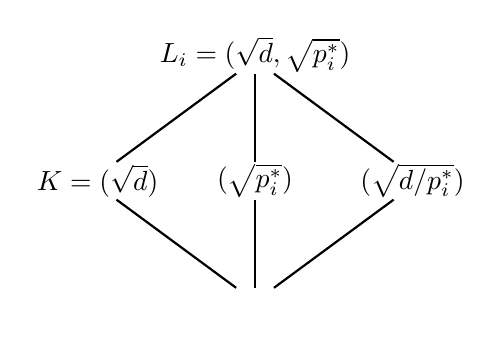
\begin{tikzpicture}[
    scale=.4,
    every node/.style={color=black}
    ]
    \node at (0,0) {$\Q$};
    \node at (-5,4) {$K = \Q(\sqrt{d})$};
    \node at (0,4) {$\Q(\sqrt{p_i^*})$};
    \node at (5,4) {$\Q(\sqrt{d/p_i^*})$};
    \node at (0,8) {$L_i = \Q(\sqrt{d},\sqrt{p_i^*})$};
    \draw[thick] (-.6,.6)  -- (-4.4,3.4);
    \draw[thick] (0,.6)  -- (0,3.4);
    \draw[thick] (.6,.6)  -- (4.4,3.4);
    \draw[thick] (-.6,7.4)  -- (-4.4,4.6);
    \draw[thick] (0,4.6)  -- (0,7.4);
    \draw[thick] (.6,7.4)  -- (4.4,4.6);
\end{tikzpicture}
\end{center}

The field $L_i$ is the compositum of $K$ with either of the two
other quadratic subfields of $L_i$, $\Q(\sqrt{p_i^*})$ and
$\Q(\sqrt{d/p_i^*})$.  Note that $p_i$ is the only finite prime
ramifying in $Q(\sqrt{p_i^*})/\Q$, so no other finite prime can
be ramified in $L_i/K$.  However, $p_i$ does not ramify in
$\Q(\sqrt{d/p_i^*})$ and, hence, does not ramify in $L_i/K$.
Thus, for each $1 \leq i \leq k$, the extension $L_i/K$ is
unramified at all finite primes.  Furthermore, $L_i/K$ is a
degree 2 extension so is abelian.  Let $L$ denote the compositum
of all the $L_i$ so that
$$
L = \Q(\sqrt{d}, \sqrt{p_1^*}, \ldots, \sqrt{p_k^*})
$$
Then $L/K$ is an abelian extension of $K$ which is unramified at
all finite primes.  If $d \equiv 2$ or $3 (\mathrm{mod} \; 4)$,
then we see that $L/K$ is an extension of degree $2^k$.
On the other hand, if $d \equiv 1 (\mathrm{mod} \; 4)$, we see
that $L/K$ is an extension of degree $2^{k-1}$.  In either case,
$L/K$ is an abelian extension of degree $2^{t-1}$ which is
unramified at all finite primes of $K$ (recall that $t$ is the
number of odd primes dividing $d_K$).

Let $\mathfrak{m}_{\infty}$ denote the modulus which is the product of all
real primes of $K$ so that the corresponding ray class group is $\Cl^+(K)$,
the narrow (or strict) class group of $K$.  It follows from class field
theory that $L$ is contained in the ray class field of $K$ corresponding to
$\mathfrak{m}_\infty$ and, thus, that $\mathrm{Gal}(L/K)$ is isomorphic to a
quotient of $\Cl^+(K)$.  So, in particular, $2^{t-1}$ divides the order of
$\Cl^+(K)$.  Let $U_K = \O_K^\times$ denote the units of $\O_K$ and let
$U_K^+$ denote the totally positive units of $\O_K$.  Then there is an exact
sequence:
$$
1 \rightarrow U_K/U_K^+ \rightarrow \prod_{v|\mathfrak{m}_\infty} \{\pm 1\}
\rightarrow \Cl^+(K) \rightarrow \Cl(K) \rightarrow 1
$$
If $d < 0$, $K = \Q(\sqrt{d})$ has no real primes and we see that $\Cl^+(K)$
and $\Cl(K)$ are the same.  If $d > 0$, $K$ has two real primes.
Dirichlet's Unit Theorem tells us that $U_K \approx \{\pm 1\} \times \Z$.
Let $\varepsilon$ be a fundamental unit of $K$: i.e., let $\varepsilon \in
U_K$ such that $U_K = \langle\pm \varepsilon\rangle$.  Then $U_K^+ = \langle
\varepsilon\rangle$ or $U_K^+ = \langle\varepsilon^2\rangle$.  Hence, the
quotient $U_K/U_K^+$ has order 2 or 4.  It follows that $\Cl^+(K)$ has order
either $2h_K$ or $h_K$ and, hence, that $2^{t-2}$ always divides $h_K$.
\end{proof}

%Simon Spicer: Added a brief section on Falting's Theorem (2013-10-03)
\section{Falting's Theorem}\label{sec:faltings}
Let $f(x,y)=0$ be a smooth plane curve. If we
consider the set of solutions to this equation over
the complex numbers there is the natural notion of
the {\it genus} of the curve: basically, the number
of holes in the solution set, when the solution set
is viewed as a Riemann surface. Genus one curves, for
example, topologically look like doughnuts. \\

It turns out that the number of rational points on a
plane curve -- that is, the number of pairs of
rational numbers $(x,y)$ that satisfy $f(x,y)=0$ --
is highly dependent on the genus of the curve
described by $f$. Genus zero curves are generally
well understood: the solution set to $f(x,y)=0$ is
either empty, or it is infinite and described by a
single parameter. \\

Genus one curves (modulo some extra conditions) are
known as {\it elliptic curves}, and are the central
objects of study in a large part of modern-day number
theory. These will be discussed in later sections and
chapters of the book, but the gist of the matter is
that elliptic curves can have wildly varying numbers
of rational points depending on the curve, from zero
to infinity and everything in between; there is an
entire industry dedicated to computing just how many
points a particular elliptic curve has. \\

Curves of genus two and above, on the other hand, are
a completely different affair.

\begin{theorem}
Any smooth projective curve of genus two or greater
has only finitely many rational points.
\end{theorem}

This is known as {\it Falting's Theorem}, after the
German mathemetician Gerd Falting who proved it in
1983 (for which he won a Fields Medal). The theorem
is in fact more general than stated above: given any
fixed number field $K$, the number of $K$-rational
points on a smooth projective curve $C$ of genus at
least two is finite. \\

Unfortunately, Falting's Theorem is completely non-constructive:
while it tells you that there will only ever be
finitely many rational solutions to an equation
describing a genus two or above curve, in no way does
it outline how to go about finding those points. In
fact, there is no general method known to find points
on curves of higher genus; nor is it even known -- or
even suspected -- if such a method exists or doesn't
exist. The question, as they say, is wide open. \\

It thus shouldn't be a surprise that the question of
finding points on higher genus curves is in itself an
active area of research in number theory. As an
example, in Diophantus' Arithmetica, the series of
books on solving algebraic equations by the ancient
Greek mathematician, there is only one instance of a
higher genus curve being considered: problem 17 of
book 6 boils down to finding rational points on the
genus two curve described by
\[ y^2 = x^6 + x^2 + 1 \]
Because of Falting's Theorem we know that this
equation only has finitely rational solutions. Two
obvious solutions are $(x,y) = (0,\pm 1)$, while
Diophantus himself gave the more interesting solution
$(\frac{1}{2},\pm \frac{9}{8})$. This single equation
is the entire topic of the PhD thesis of Joe
Wetherell (UC Berkeley 1998) \cite{wetherell1997bounding}, which uses some pretty
hefty algebraic geometry to show that no other
solutions exist. \\


\section{Fermat's Last Theorem}\label{sec:fltintro}
Fermat's Last Theorem -- a problem from the 1600s! -- asserts
that whenever $n\geq 3$, then there are no positive integer
solutions to the Diophantine equation
$$
X^n + Y^n = Z^n.
$$
This seemingly approachable problem has a long and colorful
history.
When $n=3$ the equation is
$$
X^3 + Y^3 = Z^3,
$$
which is the (projective homogenous) equation of the plane cubic algebraic
curve $x^3 + y^3 = 1$:
\begin{lstlisting}
%var x y
implicit_plot(x^3 + y^3 == 1, (x,-2,2), (y,-2,2))
\end{lstlisting}
\begin{center}
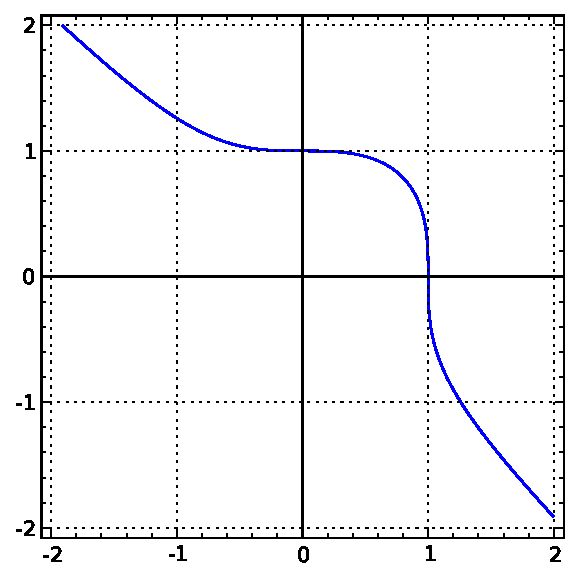
\includegraphics[width=.5\textwidth]{pics/flt3.pdf}
\end{center}
This is an example of an elliptic curve; you should
see some rational points on it---namely $(1,0)$ and $(0,1)$---these
correspond to torsion points on the elliptic curve, and to solutions
to the Fermat equation with $X$ or $Y$ equal to $0$.

For general $n\geq 5$, Fermat's assertion was finally resolved by much modern
work in number theory, culminating with a major theorem of
Andrew Wiles.  The basic strategy, which is useful for
attacking a wide range of Diophantine equations, is as follows.
Given a specific counterexample
$a^n + b^n = c^n$ to Fermat's claim (with say $n$ prime), we associate
an elliptic curve (the ``Frey curve'')
$$
  E: \quad y^2 = x(x-a^n)(x+b^n).
$$
By counting solutions modulo $p$ to the equation that defines this curve (or
any nonsingular curve of the form $y^2=x^3+\alpha x + \beta$ for that matter),
we define an $L$-series
$$
L(E,s) =
\prod_{p \text{ prime}} \frac{1}{1-a_p p^{-s} + \varepsilon(p)\cdot p^{1-2s}}
 = \sum_{n\geq 1} \frac{a_n}{n^s},
$$
where $\varepsilon(p)=1$ if $p\nmid abc$ and $\varepsilon(p)=0$ otherwise,
and $a_p = p+1-\#E(\F_p)$.
Old work of Hasse (and others)
shows that this $L$-series defines a complex analytic
function on some right half plane; people then conjectured (and
subsequently proved!)
that $L(E,s)$ extends to a holomorphic function on all $\C$.
Birch and Swinnerton-Dyer even went so far as to conjecture
that most everything about the arithmetic of $E$
is determined by the leading coefficient of the
Taylor expansion of $L(E,s)$ about $s=1$.

To the $L$-series $L(E,s)$, one can use
Mellin transform to define another complex analytic function
on the upper half plane
$$
f(z) = \sum_{n\geq 1} a_n e^{2\pi i z} = \sum_{n\geq 1} a_n q^n,
$$
where the coefficients $a_n$ here are exactly the same as
in the Dirichlet series representation of $L(E,s)$ above.
Andrew Wiles (and Richard Taylor) proved \cite{wiles:fermat}---using
an ingenious
argument involving an arithmetic analogue of Barry Mazur's
deformation theory---that
$f(z)$ has the property that for
all $2\times 2$ integer matrices
$\gamma$ with determinant $1$ and lower left entry divisible
by $N=\prod_{\ell\mid abc} \ell$, we have
$$
  f(z) dz = f(\gamma(z)) d(\gamma(z)),
$$
where $\gamma$ acts on the upper half plane
via linear fractional transformations.  This function
$f(z)$ is called a weight 2 cuspidal {\em modular form}.

Moreover, using arithmetic with {\em quaternion algebras} and
geometry of modular curves, Ken Ribet had earlier proved that
the coefficients $a_n$ of the expansion of
$f(z)$ must be congruent to the coefficients
of a cuspform of ``level 2'', which is
impossible, since there are no such nonzero forms.
This contradiction proves Fermat's last theorem.

We can explicitly compute with many of the
objects---elliptic curves, modular forms, etc.---appearing
in the discussion above.
For example, we do some computations with the elliptic
curve corresponding to Fermat's equation for exponent $n=3$
(this is {\em not} the corresponding Frey curve, but another
model for $X^3+Y^3=1$)
\begin{lstlisting}
sage: E = EllipticCurve([0,0,1,0,-7]); E
Elliptic Curve defined by y^2 + y = x^3 - 7 over Rational Field
sage: E.anlist(20)
[0, 1, 0, 0, -2, 0, 0, -1, 0, 0, 0, 0, 0, 5, 0, 0, 4, 0, 0, -7, 0]
sage: L = E.lseries(); L
Complex L-series of the Elliptic Curve defined by y^2 + y = x^3
over Rational Field
sage: L(1)
0.588879583428483
sage: L.taylor_series(1, 5)
0.59 + 0.45*z - 0.19*z^2 + 0.0042*z^3 + 0.033*z^4 - 0.018*z^5 + O(z^6)
sage: E.rank() # proves FLT for exponent 3
0
\end{lstlisting}
By computing the ranks of twists of $E$ we can tell whether or
not $E$ has infinitely many rational points over the quadratic
field $\Q(\sqrt{d})$, for various $d$.  Running this code:
\begin{lstlisting}
for d in [-5..5]:
    if d.is_squarefree() and d != 1:
       print d, E.quadratic_twist(d).rank()
\end{lstlisting}
yields:
\begin{lstlisting}
-5 1
-3 0
-2 1
-1 0
2 1
3 0
5 1
\end{lstlisting}

This means, e.g., that in the field $\Q(\sqrt{5})$, generated by
the golden ratio, there are infinitely many triples of coprime integers
$X,Y,Z$ such that $X^3 + Y^3 = Z^3$! The following code gives a few of these triples:
\begin{lstlisting} %Added by Travis Scholl
sage: R.<x,y,z> = QQ[sqrt(5)][]
sage: f = EllipticCurve_from_cubic(x^3+y^3-z^3,[-1,1,0]).inverse();
sage: for i in range(1,6):
        r = f(i*f.domain().gens()[0]); r.clear_denominators(); r
\end{lstlisting}
which outputs:
\begin{lstlisting}
(-sqrt5 + 9 : sqrt5 + 9 : 12)
(2761*sqrt5 + 225 : -2761*sqrt5 + 225 : 3720)
(-3105301*sqrt5 + 6666948 : 3105301*sqrt5 + 6666948 : 13610574)
(7206070204127*sqrt5 + 4735673343225 :
    -7206070204127*sqrt5 + 4735673343225 :
    19652111284080)
(-45203693464083879145*sqrt5 + 25364447357048949231 :
    45203693464083879145*sqrt5 + 25364447357048949231 :
    116655528338821919868)
\end{lstlisting}


% Bharath added this part - I am confused as to why we initially talked about group extensions
% william -- it was simply a "first idea" i had during the lecture; sometimes first ideas are totally useless, especially mine :-)
% Bharath: Was the goal to prove something like - every fermat triple in the field Q(sqrt 5) of a certain form - (x, sigma(x), natural number)?
% William: NO -- it was to understand why that pattern appeared in the examples that were being displayed in the presentation.  It was because he was computing triples coming from the Galois invariant subgroup.  When Thomas later considered a non-invariant subgroup, he found triples not of that form.  So it's just about explaining that observation.
% (BY THE WAY -- there is a chat on the right side -- click the message bubble)


We have a short exact sequence
\begin{align} \label{seq}
0 \rightarrow E(\Q) \rightarrow E(\Q(\sqrt{5})) \rightarrow E(\Q(\sqrt{5})) / E(\Q)  \rightarrow 0.
\end{align}
Using Sage, we can compute the torsion and rank of each group. One obtains that $E(\Q) \cong \Z/3\Z$ and $E(\Q(\sqrt{5})) \cong \Z/3\Z \oplus \Z$. The group $G$ acts on $E(\Q(\sqrt{5})) / E(\Q)$ by $-1$. One can ask the question - is there an element $x$ in $E(\Q(\sqrt{5}))$ on which $G$ acts by $-1$ and such that $E(\Q(\sqrt{5})) \cong \Z \cdot <x> \oplus E(\Q)$ (where the isomorphism is in the category of $\Z[G]$-modules).
Let us write $E(\Q(\sqrt{5})) \cong \Z \oplus \Z/3\Z$ (where the isomorphism is simply in the category of abeian groups).
Let $b$ be an element of $\Z/3\Z$ such that $\sigma (1,0) = (-1,b)$. Then one sees that $\sigma\cdot (1,b) = -(1,b)$.
One can choose $x$ to be $(1,b)$.





And we can explore the $L$-series itself:

\begin{lstlisting}
sage: h = L.dokchitser(prec=200)
sage: complex_plot(h, (-2,3), (-5,5), plot_points=10)  # quite painful
\end{lstlisting}

\begin{center}
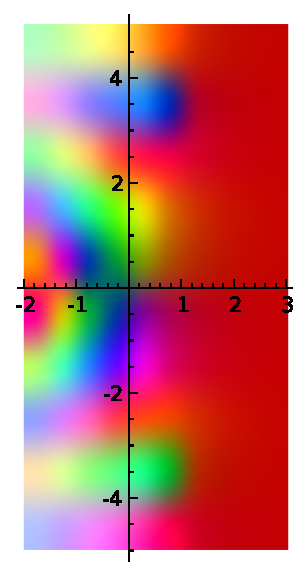
\includegraphics[width=.4\textwidth]{pics/27a-lser1.pdf}
\end{center}

As for the Riemann zeta function, there is a generalized Riemann
Hypothesis, which postulates that the nontrivials zeros of
$L(E,s)$ lie on a line, the line $\Re(s)=1$.
The first few imaginary parts of the nontrivial zeros of $L(E,s)$ are
\begin{lstlisting}
sage: L.zeros(5)
[4.04304401, 6.04893540, 8.21765037, 9.42919921, 10.9087283]
\end{lstlisting}

The general structure of Wiles's approach also generalizes to many other
Diophantine equations.  Instead of obtaining a single congruence with
forms in a space of dimension 0, we instead considers a potential
large collection of spaces of modular forms, which we systematically
compute (e.g., using modular symbols).

\subsection{Extending Fermat's Last Theorem} %Added by Travis Scholl

There are many rings where Fermat's Last Theorem fails for many values of
$n$. For example consider the ring $\Z[\zeta]$ where $\zeta$ is a primitive
$m$th root of unity with $3 | m$. Then $\xi := \zeta^\frac{m}{3}$ is
a primitive $3$rd root of unity so it satisfies $1+\xi+\xi^2=0$.
From this it is easy to see
$$
(\xi)^{6k+5} + (\xi^2)^{6k+5} = (-1)^{6k+5}
$$
for any non-negative integer $k$. Hence the triple $(\xi,\xi^2,-1)$ satisfies
the Fermat equation $X^{6k+5}+Y^{6k+5}=Z^{6k+5}$ in the ring $\Z[\zeta]$. \\

In general, it is straightforward to construct counterexamples to FLT
of degree $d$ with degree $d$ number fields: \\
Let $d\ge 3$ be a positive integer, and pick any two positive integers
$Y$ and $Z$ with $Y<Z$. Let $K = \Q(\alpha)$, where $\alpha$ obeys
$\alpha^d = Z^d-Y^d \in \Z$. Then clearly $(\alpha,Y,Z)$ is a Fermat triple lying in $K$. \\

% Added by Igor Tolkov
However, it is still possible to extend Fermat's Last Theorem to number fields. Olivier Debarre and Matthew Classen \cite{deb-cla} extend the results of Faltings to show, in particular:
\begin{theorem}[Debarre-Classen]\label{th:dc}
The equation $x^n+y^n=z^n$ has only finitely many solutions $(x,y,z)$,
where $(x,y,z)$ lie in any field of degree $d\leq n-2$.  (So we're
considering solutions in all of these fields simultaneously.)
\end{theorem}

The theorem states that there are only a few counterexamples to Fermat's Last Theorem for each exponent $n$, except over number fields of degree $n-1$ or greater. Frazer Jarvis and Paul Meekin \cite{jar} take a guess as to what these counterexamples are:
\begin{conjecture}[Jarvis-Meekin]\label{conj:jarv}
Let $K$ be a number field of degree $d$ and $n\geq d+2$. Then any solution $(x,y,z)$ over $K$ to $x^n+y^n=z^n$ satisfies $x+y=z$.
\end{conjecture}

\section{The ABC Conjecture}
The abc conjecture
concerns triples of coprime positive integers $a,b,c$  such that
$$
a+b = c.
$$
The {\em radical} of an integer $n$ is the product
of the distinct prime divisors of $n$, and the radical
of an abc triple $a,b,c$ is $r=r(a,b,c)=r(abc)$.
For example,
$$
  1 + 8 = 9
$$
has radical $r=2\cdot 3=6$.

\begin{conjecture}[Masser-Oesterl\'{e}]\label{conj:abc}
For every $\eps>0$ there are only finitely many
triples $a,b,c$ of coprime positive integers such
that $a+b=c$ and $r^{1+\eps}\leq c$,
where $r=r(a,b,c)$.
\end{conjecture}

Given $a,b$ it is trivial to find $c$ with $a+b=c$, and
usually the radical $r=r(a,b,c)$ is going to be bigger
than $c$.   A typical example is $a=4$, $b=15$.
We have $c=4+15=19$, and the radical is
$$2\cdot 3\cdot5\cdot19=570 \gg 19.$$
For the radical to be small compared to $c$
is quite special.

Now suppose for the moment that we have a counterexample
to Fermat's Last Theorem (see Section~\ref{sec:fltintro} above),
say
$$
 A^n + B^n = C^n,
$$
with $A,B,C$ coprime positive integers and $n\ge 5$ (say).
Letting $a=A^n, b=B^n, c=C^n$, we have
$$
r(a,b,c) = r(A^n,B^n,C^n) = r(A,B,C) \leq ABC <C^3 < C^n=c.
$$
According to Conjecture~\ref{conj:abc} (with
any choice of $\eps$), there can be only finitely many such
triples $(A^n, B^n, C^n)$.  In particular, Conjecture~\ref{conj:abc} implies
Fermat's Last Theorem for all sufficiently large $n$.
\footnote{An accepted proof of FLT is known (due to Wiles). There
is no accepted proof of ABC, but there is a claimed one,
which may or may not be right...
\begin{quote}
``The problem with wrong proofs to correct statements is that it is hard to give a counterexample.'' -- Hendrik Lenstra, \url{http://www.ucs.louisiana.edu/~avm1260/lenstra.html}
\end{quote}}

There's much computational work that goes into understanding
and refining the ABC conjecture.  For example,
Lenstra defined a notion of the {\em quality} of
a triple $a+b=c$ to be
$$q(a,b,c) = \frac{\log(c)}{\log(r)}.$$

Here is a Sage interact to compute the quality:
\begin{lstlisting}
@interact
def f(a=3, b=4):
    c = a + b
    print "%s + %s = %s"%(a,b,c)
    v = prod(set(prime_divisors(a) + prime_divisors(b) + prime_divisors(c)))
    q = log(c)/log(v)
    print "quality = ", float(q)
\end{lstlisting}

Notice that if we chose $\eps$ to get equality
in Conjecture~\ref{conj:abc}, then
$q(a,b,c) = 1+\eps$.
As mentioned above, triples $a,b,c$ usually have
very low quality, since
$r$ is typically much bigger than $c$.
However, there are some known triples $a,b,c$ of
high quality, but the ABC conjecture asserts there aren't too
many.  In fact, here is an equivalent version of the ABC conjecture:
\begin{conjecture}
For every $h>1$ there are only finitely many triples
$a,b,c$ with quality bigger than $h$.
\end{conjecture}

The highest quality triple ever found\footnote{See \url{http://www.math.leidenuniv.nl/~desmit/abc/}.} is
$
   2 + 3^{10}\cdot 109 = 23^5,
$
where
$$
q(a,b,c) = \frac{\log(23^5)}{\log(2\cdot 3 \cdot 109 \cdot 23)}
    = 1.62991168412\ldots
$$

Even if you don't believe the ABC conjecture, you might believe this:
\begin{conjecture}[Weak ABC]
Among all $a,b,c$ triples, there is an absolute upper
bound on the quality.
\end{conjecture}

\begin{exercise}
Does the above weaker conjecture imply Fermat's Last Theorem for all sufficiently large exponents $n$?
\end{exercise}

\begin{exercise}
If possible, formulate ABC over number fields in terms of a notion of ``quality''.  See \url{http://www.math.columbia.edu/~goldfeld/ABC-Conjecture.pdf} for a precise statement of ABC over number fields.
What does this imply about FLT over number fields?
\end{exercise}

%added by Hao Chen 10/6/13
In the paper mentioned in Exercise 1.5.5, Goldfeld
formed a slightly different version of ABC: \\

(ABC')Let $A,B,C$ be nonzero, coprime integers such that
$A+B+C = 0$. Let $N = \prod_{p \mid ABC} p$.
Then for every $\epsilon >0$, there exists $\kappa(\epsilon)>0$
such that
\[ \max(|A|,|B|,|C|) < \kappa(\epsilon) N^{1+\epsilon} \]
The first question is if this conjecture is equivalent
to ABC. One sees that ABC implies ABC': indeed, fix
any $\epsilon >0$, then $\kappa$ can be chosen to be any number greater than $\max\{ \frac{\max\{|A|,|B|,|C|\}}{N^{1+\epsilon}}\}$. This maximum taken over a set is finite since by ABC all but finitely many element in
this set is smaller than 1. \\

Proof that ABC' implies ABC: Fix $\epsilon > 1$,
choose $\delta$ s.t. $\epsilon > \delta > 1$, then
by ABC', there exists some positive constant $\kappa(\delta)$
such that $\max(|A|,|B|,|C|) < \kappa(\delta) N^{1+\delta}$
holds for all triples. Now for any triple s.t. $N^{1+\epsilon} < \max(|A|,|B|,|C|)$ we have
$N^{1+\epsilon}< N^{1+\delta}$, which can only hold for
finitely many $N$. Hence $N$ is bounded above, and we see
from ABC' that $\max(|A|,|B|,|C|)$ is bounded above. So
there's finitely many such triples. \\

%added by Hao Chen --10/14/13: abc conjecture for number fields.

To generalize this to number field, one needs to extends
the notion of absolute value and radical by the following:
Let K be a number field and $V_K$ denotes the set of primes
of K. Define
\[
    H_K(a,b,c) = \prod_{v \in V_K} \max\{|a|_v,|b|_v,|c|_v\}
\]
and
\[
    rad_K(a,b,c) = \prod_{P \in IK(a,b,c)}N_{K/\mathbb{Q}}(P)
\]
where $I_K(a,b,c)$ is the set of all prime ideals $P$ of OK for which $|a|_v,|b|_v,|c|_v$ are not equal. The abc conjecture for K states that for any $\epsilon >0$,
there exists $\kappa(\epsilon, K)>0$
such that
\[
H_K(a,b,c) < \kappa(\epsilon, K) rad_K(a,b,c)^{1+\epsilon}
\]

\subsection{Infinitely many triples with quality greater than $1$}
For $p$ an odd prime and $n\geq 1$ an integer, consider the $a,b,c$ triple
$$
a = 1,\qquad b = 2^{p(p-1)n}-1, \qquad c = 2^{p(p-1)n}.
$$
Since $\varphi(p^2)=p(p-1)$ is the order of $(\Z/p^2\Z)^*$,
we have $2^{p(p-1)n}\equiv 1 \pmod{p^2}$,
so $p^2 \mid b$.
Thus
$$
 r = r(a,b,c) = 1 \cdot p \cdot\text{(other stuff from $b$)} \cdot 2
     \leq \frac{2b}{p} < b < c,
$$
so
$$
 q(a,b,c) = \frac{\log(c)}{\log(r)} > 1.
$$
Here is a Sage interact to compute $a,b,c$ as above, along with their quality.
Note that if you put at all largve values in for either $n$ or $p$,
then the resulting numbers are huge, and the computation of the quality
(as implemented) will take forever.
\begin{lstlisting}
@interact
def f(p=3, n=1):
    if not is_prime(p) or p<=2:
        print "p must be an odd prime!"
    if n < 1:
        print "n must be >= 1"
    a = 1
    b = 2^(p*(p-1)*n) - 1
    c = 2^(p*(p-1)*n)
    print "%s + %s = %s"%(a,b,c)
    print "(now computing quality...)"
    sys.stdout.flush()
    v = prod(set(prime_divisors(a) + prime_divisors(b) + prime_divisors(c)))
    q = log(c)/log(v)
    print "quality = ", float(q)
\end{lstlisting}

\subsection{Triples with Quality at least $1.4$}\label{sec:abchome}
The following is a plot of the number of abc triples with $c\leq 10^x$
and quality at least $1.4$, drawn on a log scale,
where $x\leq 10^{18}$.  This data was computed by the ABC@HOME project.
\begin{center}
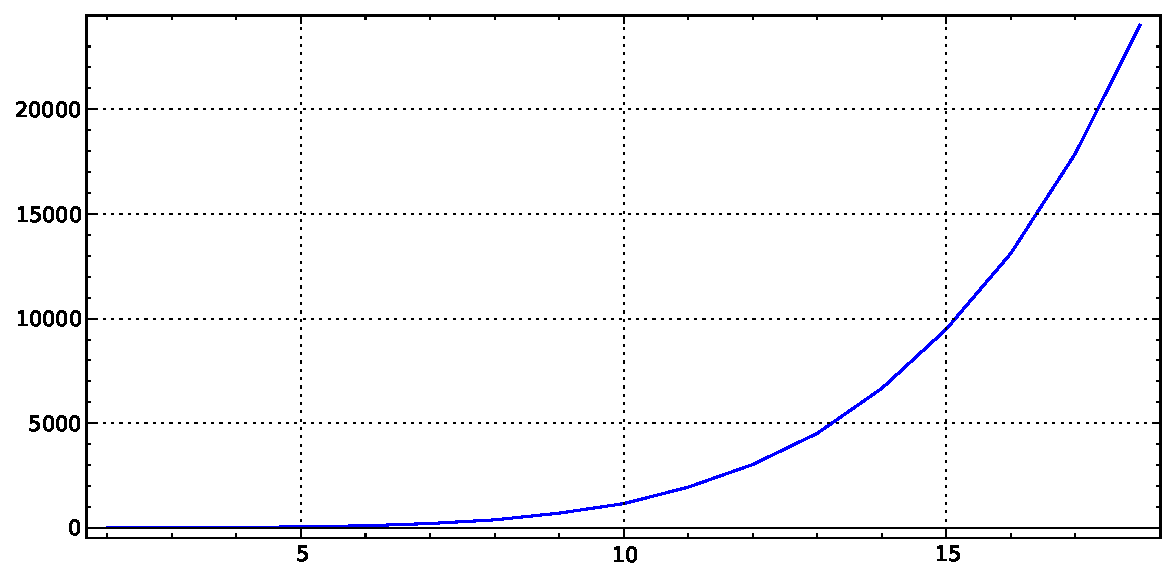
\includegraphics[width=.7\textwidth]{pics/abcplot.pdf}
\end{center}

The (strong) ABC conjecture asserts that the blue line is bounded above!
As is typical is typical with most questions in "asymptotic number theory",
the numerical data suggests---to the naive observer---the exact opposite.
See \cite{bmsw:bulletins} for an article about this sort of tension in
another context:
\begin{quote}
``We have a network of heuristics and conjectures regarding rational points, and we have massive data accumulated to exhibit instances of the phenomena. Generally, we would expect that our data supports our conjectures; and if not, we lose faith in our conjectures. But here there is a somewhat more surprising interrelation between data and conjecture: they are not exactly in open conflict one with the other. We discuss various aspects of this story, including recent heuristics and data that attempt to resolve this mystery.''
\end{quote}

{\bf Student Project Idea: (Andrew Ohana is mainly doing this)} {\em Completely forget about the ABC
conjecture, pretend you are an applied mathematician,
and model the function that counts the number of ABC
triples of quality $q$ up to $10^x$.}
\begin{enumerate}
\item Beg, barrow, or steel the complete dataset from the ABC@Home
project.  This could be pretty challenging, since currently their
site is down with ``{\tt Warning: mysql\_pconnect(): Too many connections in /data/project/abc/html/inc/db.inc on line 39...}''.  That said, I know the people who run this site,
and we can contact them directly.
\item For a few hundred values of $q$ with $1\leq q\leq 1.67$,
use the data to "compute or plot" the function
$$
f_q(x) = \#\{\text{number of ABC-triples with $c<10^x$
of quality $\geq q$}\}.
$$
The plot will look like the blue curve above.
\item
Use various models of your choosing to find a smooth
function that best fits that curve?  Your smooth
function will be parametrized by $q$, i.e., you get
a different function for each value of $q$.
I don't have any idea what sort of function to expect.
A polynomial?  Exponential?  Something else?  Note that
according to the ABC conjecture, the function $f_q(x)$
is supposed to be {\em bounded above} for each $q>1$!
(However, just pretend you don't know about that and you're
a physicist or something....)
\item What happens if you let the parameter $q$
in the above model go to $\infty$?
\item Can you find a different model for $f_q(x)$ that
{\em is} bounded above (hence consistent with the ABC
conjecture), and also fits the data?
\end{enumerate}

The above seems to me to be the most obvious first thing to
do if one had computing power and wanted to make the ABC
conjecture in the first place.  However, the data to do the
above computation wasn't available until very recently,
so maybe nobody did it (which I find sort of shocking if true).

% Bharath added this section
\section{Some consequences of the ABC conjecture}

\begin{enumerate}
\item In \cite{ichimura1998note}, assuming the generalized ABC conjecture for number fields, H. Ichimura shows that for a given real quadratic field $k$, there exists infinitely many prime numbers $p$ such that the Iwasawa $\lambda$-invariant is 0.
%[[is 0 -- this was blank?? -- William]]
This is closely related to Greenberg's conjecture.
\item In \cite{elkies1991abc}, N. Elkies shows that the generalized ABC conjecture for number fields implies the Mordell conjecture.
\end{enumerate}


\section{Public-key Cryptography}


\begin{quote}
``Nowadays, when a Number Theorist applies for a grant, he says
that Number Theory is used in cryptography, and so doing Number
Theory is good for National Security. Back then, since it was
before the discovery of America, they said Number Theory is
used in music. But I won't comment on the progress of
civilization since then.''\\-- Hendrik Lenstra,\\ \url{http://www.ucs.louisiana.edu/~avm1260/lenstra.html}
\end{quote}


Public-key cryptography involves many of the same ideas and tools
as the rest of computational number theory, and so in this book
we will consider it on an equal footing.
In particular, we will consider the RSA cryptosystem, whose
security relies on the difficulty of factoring integers,
and also elliptic curve-based cryptosystems
such as ElGamal and elliptic curve Diffie-Hellman.

There are two intimately related sides to cryptography:
creating methods to send encrypted messages,
and cracking proposed encryption methods.
It's extremely difficult to be good at
creating methods for encrypting messages, but
bad at attacking them, since one must be very aware of
attack techniques in order to guard against them.
It's probably less important to be good at making encryption
systems if you want to be good at cracking them.
It is natural that the typical cryptography group at a big
company would put more effort into
creating and implementing cryptosystems than into attacking them,
since they
have little commercial motivation for investing billions
into attacking cryptosystems,
and publicity about them doing so probably wouldn't look
good (and indeed, such attack technology might have legal implications).
\begin{quote}
``Former NSA technology boss Prescott Winter has a word for the kind of security he sees even at large, technologically sophisticated companies: Appalling''\\
 -- \url{http://tinyurl.com/pgb45j8}, Slashdot, Oct 3, 2013.
\end{quote}

For the cryptography aspect of this course, we'll consider the cryptosystems above, and some of the attacks on them, and how all of this work
has a deep interplay with many other objects we consider.

% NEWS: https://news.ycombinator.com/item?id=6506120

\subsection{The Standard Protocols}
To get started, let's quickly go over a couple of bog
standard public-key cryptography protocols: Diffie-Hellman,
RSA, and elliptic curve ElGamal.

\subsubsection{Diffie-Hellman}
The Diffie-Hellman key exchange protocol enables two
programs $A$ and $B$ to agree on a common secret in full view of an
adversary.   For example, Diffie-Hellman (but on an elliptic curve)
is used  when you connect your web browser to the
\url{https://cloud.sagemath.com} website in order to agree
on a secret key that is used to encrypt all further data.

Here's how it works.
\begin{enumerate}
\item Programs $A$ and $B$ agree on a prime number $p$ and a primitive
root $g$ modulo $p$, i.e., a number that generates $(\Z/p\Z)^*$.
\item Program $A$ compute a random number $a$ and program
$B$ computes a random number $b$.
\item Program $A$ sends $g^a\pmod{p}$ and program $B$
sends $g^b\pmod{p}$.
\item Program $A$ and program $B$ compute the secret
$$
   s = (g^a)^b\pmod{p} = (g^b)^a\pmod{p}.
$$
\end{enumerate}
One subtlety is that there is a fast algorithm to
compute $g^n\pmod{p}$ -- to do this, write $n$
in binary, and compute $g\cdots g$ ($n$ times)
by a couple of repeated squarings, reducing
modulo $p$ at each step... which is {\em easy}.

The main theoretical assumption one makes is that given $g^n\pmod{p}$
and $g\pmod{p}$ it is ``difficult'' to compute $n$, i.e., to find
$\log_g(g^n \pmod{p})$.  This is the {\em discrete log problem}.
There are some primes $p$ for which this assumption is obviously
false.  For example, if $p-1$ factors as a product of many small
numbers, then solving the discrete log problem in $(\Z/p\Z)^*$ is
no more difficult than solving it in groups with these much smaller
orders, hence easy.   So, if when using Diffie-Hellman, it is critical
to check that $p-1$ doesn't factor too much; the best you can hope
for is that $p-1 = 2q$, with $q$ prime, and this is what people
often use.

 See Section~\ref{sec:primroot} below for a discussion of
 the complexity of finding a primitive root.

Once you commit to seriously using Diffie-Hellman modulo a prime, you have
to worry about how big to make $p$.  If you make $p$ enormous, then
everything takes more memory and is slower.  For example, for large $p$
establishing a connection to \url{https://cloud.sagemath.com} might
take so much time (seconds!) that you'll just loose patience.  To decide
how big a $p$ to take, you basically have to learn about algorithms for
attacking the discrete log problem, look at what challenge problems
people have solved in practice, then bet the farm on a particular
choice size of $p$.    In practice, people usually trust organizations
such as NIST (which is advised by NSA, which knows a thing or two)
to make the decisions for them.

\begin{exercise}
How big of primes $p$ to people actually use?
\end{exercise}

There is an algorithm called "baby-step giant-step" which can solve
the discrete logarithm mod $p$ using time and space $O(\sqrt{p})$; we'll
consider this algorithm in more detail later, since it is extremely
important in computational  number theory.


The Diffie-Hellman key exchange is amenable to the {\em man-in-the-middle
attack}, where an adversary intercepts all transmissions, and
agrees on two different secrets, one with program $A$ and a {\em different
secret} with program $B$.  Then the adversary decrypts/encrypts
all traffic between $A$ and $B$.  This is not theoretical -- exactly
this attack is used successfully
in practice on the Internet (see recent news articles).


\subsubsection{RSA}
The RSA cryptosystem allows a program $A$ to publish a public key
for all to see. Any program $B$ can then send $A$ a message that is encrypted
using this public key.  Also, $A$ can sign documents
using their corresponding private key, and $B$ can use
$A$'s public key to verify that indeed $A$ signed the document.
This RSA solves two problems: (1) being able to encrypt a message to $A$
without any specific activity on $A$'s part (unlike with Diffie-Hellman),
and (2) being able to digitally sign a document.
The main issue is that $B$ has to trust that $A$'s public key is...
really $A$'s public key, and in practice this is a major pain.

Here's how it works.
\begin{enumerate}
\item Program $A$ chooses two prime numbers $p\neq q$
and computes $n=pq$, computes $\varphi(n) = (p-1)(q-1)$,
and chooses an integer $e>1$ that is coprime to $\varphi(n)$.
Program $A$ then publishes $(n, e)$.  Also, program $A$
computes $d$ such that $ed\equiv 1\pmod{\varphi(n)}$.
\item Program $B$ encrypts a message $m\pmod{n}$ to $A$
by computing $m^e\pmod{n}$.  (We assume the message $m$
is coprime to $n$.)
\item Program $A$ decryptes the message $m^e\pmod{n}$
by computing $m=(m^e)^d\pmod{n}$, where we use that
$\varphi(n)$ is the order of $(\Z/n\Z)^*$.
\item Also, if program $A$ wishes to sign a message $m$,
then program $A$ publishes $m$ and $m^d\pmod{n}$.
\item Program $B$ can verify that program $A$ signed $m$
by computing $(m^d)^e\pmod{n}$ and checking that this
equals $m$.
\end{enumerate}

The security of RSA relies on the secret $d$, which is easy
to compute if you know $\vphi(n)$.  However, knowing $\vphi(n)$
requires factoring $n$, which seems---as far as we know---to
be difficult in general.   All the same remarks as for Diffie-Hellman
apply above; in order to know how big to choose $n$, you need
to be intimately familiar with approaches to factoring large integers
$n$, or you look at what people have done and trust expert recommendations.
As always, there is a tradeoff between speed and security.

\begin{exercise}
Install the gpg program (``gnu privacy guard''), generate an RSA
key, and post the public part of it on your webpage, so that other
people can send you secret messages.  What bitsize did you choose?
\end{exercise}

\subsection{Elliptic Curve Cryptography}

For any prime power $q$ and any elliptic curve
$$
E: \quad y^2 + a_1 xy + a_3y = x^3 + a_2 x^2 + a_4 x + a_6
$$
with $a_1, a_2, a_3, a_4, a_6 \in \F_q$,
you can build various cryptosystems
using the abelian group $E(\F_q)$.
In 1985, Neal Koblitz and Victor Miller were the first to really
push this idea in cryptography.

Elliptic curves are used {\em a lot} in cryptography
these days.  The primary motivation for using elliptic curves
instead of $(\Z/n\Z)^*$ or $\F_q^*$ is that... professionals
tell us to.  More precisely, based on guesswork and
the ability of attackers, there's a belief that to get
``sufficient security'' using elliptic curves involves
much smaller key sizes than getting the same security
using $(\Z/n\Z)^*$ or $\F_q^*$.  These smaller key sizes
result in faster protocols -- e.g., connecting to a secure
webpage is faster, or the license key you
type in when installing software is much shorter.

\subsubsection{Diffie-Hellman on an Elliptic Curve}
Instead of choosing a primitive root $g$ in $(\Z/p\Z)^*$,
choose a point $G \in E(\F_q)$.  It's not critical that
$G$ generate the possibly non-cyclic group $E(\F_q)$.
Instead, it's important that $G$ have large prime order.
The fact that it is possible to efficiently compute the
order of $G$ -- even when $q$ has hundreds of digits ! --
is very deep and surprising, and is called the
Schoof-Elkies-Atkin algorithm (or SEA for short).
That this is possible is absolutely crucial to really
making elliptic curve cryptography viable.

With $G$ agreed upon, progams $A$ and $B$ publish
$aG$ and $bG$, for random secrets $a$ and $b$,
which can both be computed efficiently by writing
$a$ and $b$ as sums of powers of $2$ (i.e., in binary).
Then the shared secret is
$$
S=b (a G) = a (b G).
$$


\subsubsection{RSA on an Elliptic Curve?}
Well, let's see...  WARNING: I've never
read anything about this: I just thought it through right now -- William.

RSA relies on being able to construct and publish
an algebraic
group (in this case $\G_m(\Z/n\Z)$)
such that you know the order of the group,
but it is difficult for other people to compute
the order of that group.
If the algebraic group is an elliptic curve over
the field $\F_q$, then this is not possible,
since the SEA algorithm ensures that anybody can efficiently
compute the order of $E(\F_q)$.
A direct analogue of RSA on $E(\F_q)$ would
have public key $(E/\F_q, e)$, where $e$
is some random number modulo the exponent
of the group $E(\F_q)$.
One would encode a message as a point $M \in E(\F_q)$
then encrypt it as $e M \in E(\F_q)$.

To encode a message as a point on the curve, you of course
first break the message up into smaller pieces, add salt (randomize it somehow), then get a possible $x$ coordinate.  By solving a quadratic
equation in $\F_q$, which can be done efficiently in practice, one
constructs a point $(x,y)$, or if there are no solutions, simply slightly
modify $x$ to get a solution (since half of the $x$'s work).  Solving
a quadratic equation involves extracting a square root, which can be done
efficiently in practice (see [[reference to something]]).

However, there's a major problem with this protocol, which involves
getting confused about what the discrete log problem is.
If you know $e M$ and $e$, you can
compute $M$ by multiplying $e M$ by the multiplicative
inverse of $e$ modulo the order of $M$, and this order
is easy to compute since we know $\# E(\F_q)$.
The discrete log problem in $E(\F_q)$ is a different problem:
\begin{quote}
{\bf Discrete Log Problem: } {\em Given $M$ and $e M$, what is $e$?}
\end{quote}

Another analogue of RSA would be to generalize the
notion of elliptic curve to obtain an object
$E$ defined over $\Z/n\Z$,
where $n=pq$ is a product of distinct primes.
Using the theory of {\em group schemes} one can
put such a more general definition on a rigorous footing.
The isomorphism $\Z/n\Z\\isom \Z/p\Z \oplus \Z/q\Z$ induces
a canonical isomorphism
\begin{equation}\label{eq:ellisom}
  E(\Z/n\Z) \isom E(\Z/p\Z) \oplus E(\Z/q\Z),
\end{equation}
but (presumably it is easy to prove that)
one must factor $n$ in order to compute
this isomorphism.

\begin{exercise}
Prove (if easy/true!?) that if you know
the isomorphism \eqref{eq:ellisom}, then you
can factor $n$.
\end{exercise}

One then encrypts a message $M\in E(\Z/n\Z)$
as $e M$, which one can compute.
But wait, given a message $M$, how do you encode
it as a point on the curve?  To do so, you need to be
able to extract square roots in the ring $\Z/n\Z$.
I can't think of any way to do this without factoring $n$.
Of course, if you choose $E$ to have an obvious point
on it, then you can do lots of arithmetic to find many
other points on $E$.  However, they are all basically random---you
can only encrypt nonsense.

Incidentally, a critically important approach to
factoring an integer $n$ is to consider the
group $E(\Z/n\Z)$ for a certain choice of curve
with an easy-to-find point on it, and to do arithmetic
there, as if $n$ were prime.  If something goes wrong,
one discovers a factorization of $n$.  This is
H. Lenstra's Elliptic Curve factorization Method (ECM).
It turns out it is very good at splitting off medium
sized factors of an integer.  Given a large integer
$n$, the ECM algorithm finds primes $p\mid n$ that
are bigger than trial division finds, but usually much
smaller than $\sqrt{n}$.   I've heard that this algorithm
is crucial as an intermediate step in ``number field
sieve'' attacks on RSA itself.

\subsubsection{ElGamal on an Elliptic Curve}

The ElGamal cryptosystem makes sense in any cyclic abelian group,
and provides a way to solve some of the problems that RSA addresses.

Here's how it works.
\begin{enumerate}
\item Program A chooses an elliptic curve $E$ over $\F_q$, a point
$P\in E(\F_q)$ of large order, and computes a secret random number $a$.   Program
A then publishes the public key $(E/\F_q, P, aP)$.  The private key is $a$.
\item Program B encrypts a message $M \in E(\F_q)$ as follows.  Program B
computes a random secret integer $r$ and encrypts $M$ as the pair
$(rP,M + raP)$.
\item Program A decrypts the message by computing
$M = M + raP - arP$, which program A can compute because
it knows the secret number $a$.
\end{enumerate}

Conceptually, ElGamal is just an obvious extension of Diffie-Hellman.
Program A does its part of Diffie-Hellman
and ``puts it out there'' as a public key.
Then, program B does its part of Diffie-Hellman to construct a shared
secret -- namely $raP$ -- and just uses that shared secret as a one-time
pad to encrypt the message.

With RSA there is perfect symmetry between the public and private keys, but
with ElGamal the public key is two points on an elliptic curve and the private
key is a number.  Thus ElGamal does not naturally also produce
a way of constructing digitial signatures.

\subsection{The Elliptic Curve Digital Signature Algorithm}

The Elliptic Curve Digital Signature Algorithm (ECDSA) is a widely used
algorithm that solves---using elliptic curves---another problem that RSA solves, namely
digitally signing messages.
It is, for example, used as part of every bitcoin transaction.
As we saw above, even
with ElGamal, it is not at all obvious how to solve this problem!
ECSDA was invented by Scott Vanstone in 1992. (Speculation:
The internet suggests that
Vanstone maybe (?) invented ECDSA while working at the NSA,
then started a company called Certicom, patented some elliptic curves
then licensed the patents back to the NSA for \$25 million dollars?
And there are aliens 'n stuff.  Anyways, I'm sure Koblitz can clear this up.)


\subsubsection{The ECDSA Protocol}
Whenever we choose a random element ``of $\F_p$'' below, we choose it to be neither $0$ or $1$.

\protocol{Program A digitally signs a message $m$ using
ECDSA as follows:}
\begin{enumerate}
\item{}[Setup Protocol]
Choose a prime power $q$, an elliptic curve $E/\F_q$, and a
point $G \in E(\F_q)$ of prime order $p$ (which has nothing to do with $q$),
and define a set-theoretic map (in any way) $\phi:\F_q \to \F_p^*$.
Choose a random secret number $d \in \F_p^*$,
and let $Q=dG$.
The public key is $(E,G,Q,p)$ and the private key is $d$.
\item{}[Hash] Hash the message $m$ to an element $z\in \F_p^*$.
\item\label{ecdsa:rp}{}[Random Point] Choose a random $k\in \F_p^*$, and compute $kG \in E(\F_q)$.
\item{}[Compute Signature] Compute
$$r=\phi(x(kG))\in \F_p^*\text { and }
s=(z+r d)/k \in \F_p$$
In the unlikely case
$s=0$, choose a new random point in step~\ref{ecdsa:rp};
otherwise, the signature of the message
$m$ is the pair $(r,s)$ of elements of $\F_p^*$.
\end{enumerate}


\protocol{Program B verifies a digital signature $(r,s)$
of a message $m$ using ECDSA as follows:}
\begin{enumerate}
\item{}[Hash] Hash $m$ to the same $z\in \F_p^*$ as above.
\item{}[Verify] The signature is valid if $r=\phi(x(C))$,
where
$$C = \frac{z}{s} G + \frac{r}{s} Q \in E(\F_q).$$
Here $z/s$ and $r/s$ are the quotients in the field $\F_p$, and
we view $\langle G\rangle \subset E(\F_q)$
as a one-dimensional $F_p$-vector space.
\end{enumerate}


\begin{proposition}\label{prop:ecdsa}
If $(r,s)$ is a valid signature, then Program B will conclude that
it is a valid signature.
\end{proposition}
\begin{proof}
Suppose that $(r,s)$ is a valid signature, so
$$s = \frac{z+rd}{k} \in \F_p^*.$$
Then
$
k = \frac{z+rd}{s},
$
so
$$
k G = \frac{z}{s} G + \frac{rd}{s} G
  = \frac{z}{s} G + \frac{r}{s} Q = C,
$$
hence $\phi(x(C)) = \phi(x(kG)) = s$.

\end{proof}

\subsubsection{Playstation 3 Hacked!}

In 2010, Sony implemented ECDSA for the Playstation 3, in order to control
what PS3 owners could run on their game consoles.  Evidently, they crossed
some line, and specifically made it so people could no longer run Linux (and
pirate games) on their PS3.  So some people decided to attempt to crack
their implementatio of ECDSA.  Studying many examples, the noticed a pattern.
It turned out that instead of choosing the parameter $k$
at random in Step~\ref{ecdsa:rp} of the signature protocol, they
always used the same value of $k$!  Oops.

Why is this a problem?  Suppose we have in hand two valid
signatures $(r,s)$ and $(r',s')$ with corresponding hashed
messages $z$ and $z'$.  Recall that the private
key is some $d\in\F_p^*$, so our goal is to find $d$.
As in the proof of Proposition~\ref{prop:ecdsa}, we have
\begin{equation}\label{eqn:ecdsacrack}
\frac{z+rd}{s} = k = k' = \frac{z' + r'd}{s'}
\end{equation}
Oops, that's one linear equation in one unknown, namely the private
key $d$.  So with two signatures, one can solve for $d$, get
the private key, and it's game over.

More generally, when implementing ECDSA, it is extremely important to
choose $k$ sufficiently randomly.  If there is something sufficiently
predictable about $k$ -- even a few bits -- then one
can get information toward \eqref{eqn:ecdsacrack}, and with sufficiently
many signatures, recover $d$.


\subsection{The Bitcoin Elliptic Curve}




Bitcoin appears to be the first successful digital currency in history. It's
revolutionary, in that it is not supported or controlled by governments,
banks, or anything else real or political.\footnote{Many mainstream
institutions are threatened by bitcoin:\\ \url{http://www.coindesk.com/capital-one-closes-bank-account-bitcoin/}.  Bitcoin also makes it very difficult for powerful
governments to steal all the money of people who do things they don't like:  \url{http://www.extremetech.com/computing/168139-fbi-unable-to-seize-600000-bitcoins-from-silk-road-operator}}.
There are many aspects of how the
system works (and how bitcoins are mined), but there is one critical part that
involves computational number theory, and that's what we'll discuss.
In order to spend bitcoin, a certain message is digitally signed,
which involves computationa of a hash followed by application of the
ECDSDA algorithm.  Thus for Bitcoin, trust in governments, banks, armies,
credit ratings, etc., is replaced trust in this elliptic curve
$$
y^2 = x^3 + 7\quad\text{over}\quad \F_p,\,\,\text{where}\,\,
p=2^{256} - 2^{32} - 2^9 - 2^8 - 2^7 - 2^6 - 2^4 - 1.
$$
This curve has cardinality the 256-bit prime
\begin{align*}
\#E(\F_p) =& 11579208923731619542357098500868790785283756427907\\
& 4904382605163141518161494337
\end{align*}
The fixed base point $G$ on the curve is
\begin{align*}
G =& (550662630222773436695787188951685343262506034537775941\\
     & \quad 75500187360389116729240, \\
     & 32670510020758816978083085130507043184471273380659243\\
     & \quad 27593890433575733748242)
\end{align*}
which obviously generates $E(\F_p)$, since it generates a subgroup
of a group of prime order.

The curve $E$ and point $G$ above have the official name {\bf secp256k1}, where the
$256$ refers to the number of bits of $p$, and the $k$ is the first
letter of Neal Koblitz's last name.
This curve is somehow special in that there is a way to more cleverly compute
$kG$, which results in very real speedups in practice, as compared
to computing $kG$ on a ``generic'' 256-bit elliptic curve.  There's
an extensive discussion online about actual implementations, where
they claim a 30\% speedup in practice, while also expressing serious
reservations about using a special curve as the foundation for such
an important cryptosystem -- finding a fast way to solve the discrete
log problem on this one particular curve would have a major impact
on a billion dollar economic system.

Koblitz remarks:  ``[This speedup is described in]
Jerry Solinas' Crypto '97 talk, and is very concrete
and understandable.  It boils down to writing number in the base rho,
where $\rho=(-1+\sqrt{-7})/2$.  That talk was the first Crypto talk by an
NSA person.''


\subsubsection{Bitcoin Hacked!}
We saw above when discussing the PS3 crack that
it is critical that every single time program A signs a message
using ECDSA, that a {\em different} random value~$k$ is used.
If any $k$ is ever re-used, the private key can then be easily found.
In August 2013, exactly this problem surfaced in many of the bitcoin wallet
implementations for Android, and it was actually exploited:
\begin{quote}
``It looks as though, at least on occasion, the Java-based PRNG on Android will repeat its pseudorandom sequences, thanks to a flaw in Android's so-called SecureRandom Java class.  The Bitcoin Forum has already reported the theft of close to BTC56 (worth about US \$6000) from a number of people. A list of known-vulnerable Android Bitcoin wallets has been published by the Bitcoin Project, with instructions on what to do when the various wallet apps are fixed to use better-quality random numbers.''

\url{http://nakedsecurity.sophos.com/2013/08/12/android-random-number-flaw-implicated-in-bitcoin-thefts/}
\end{quote}

The fix for users was to create a new bitcoin public/private key pair using
a more secure approach, and transfer all of their money to themselves.


%Bharath added this section


\subsection{Finding a primitive root mod $p$}\label{sec:primroot}

In this section, a primitive root mod $p$ will refer to a  generator of the cyclic group $(\Z/p\Z)^\times$. First, let us consider an easy example.
Let us assume that the prime $p$ satisfies the relation $p-1=2\cdot q$, where $q$ is also a prime number.
Now, the order of any element in $(\Z/p\Z)^\times$ is either $1$, $2$, $q$ or $2 \cdot q$.
Now, $-1$ is not a square in $(\Z/p\Z)^\times$, since $4$ does not divide $p-1$.
Hence, either $2$ or $-2$ (and exactly one of them) will be a generator for the cyclic group $(\Z/p\Z)^\times$.
So, it suffices to computee $2^q$ and check if it equals $1$ or $-1$. A naive algorithm for finding a primitive root would be systematically computing $m^{(p-1)/2}$, for every element $m$ in $(\Z/p\Z)^\times$. If an element $m$ satisfies the equality $m^{(p-1)/2} = -1 (\mod p)$, then the element $m$ must be a primitive root.

There are polynomial time algorithms which assume the validity of the generalized Riemann Hypothesis.
For instance, in \cite{shoup1992searching}, the algorithm to find a primitive root is of order $O(\log^6(p))$. There are some polynomial time algorithms for computing primitve roots. For instance, see \cite{dubrois2006efficient}.

There are $\phi(p-1)$ generators in $(\Z/pZ)^\times$, where $\phi(x)$ is the Euler-toitent function.
If one chooses an element from $(\Z/p\Z)^\times$ at random, the probability that this element is a generator is $\phi(p-1)/(p-1)$.
Artin has conjetured that that a given integer $n$ which is not equal to $1$, $-1$ and which is not a perfect square is a primitive root for infinitely many primes $p$.
The conjecture is still open, though some progress has been made in \cite{gupta1984remark} and \cite{heath1986artin}.
Artin's conjecture gives us some hope that sampling at random will lead to a primitive root.
By the prime number theorem, $\phi(p-1)/(p-1) \sim 1/\log(p)$.
In practice, by selecting an element at random, one expects to find a primitive root after $(p-1)/\phi(p-1)$ tries, which is of order $O(\log(p))$ (which is significantly smaller than $O(\log^6(p))$).




%[[Point of this section: figure out the theoretical
%complexity of finding a primitive root,
%when $p-1=2q$ is prime, both assuming RH and not assuming RH.
%Also, there's an issue of deterministic versus non-deterministic
%algorithms.]]


\chapter{Enumerating Elliptic Curves}

The main goal in this chapter is to understand the
following deep recent theorem:
\begin{theorem}
There is an algorithm that
takes as input a positive integer $N$ and outputs all elliptic curves
defined over $\Q$ of conductor $N$.
\end{theorem}
Along the way, we'll learn many interesting theorems related
to elliptic curves and about how to compute modular forms using
modular symbols.

\begin{definition}[Elliptic Curve]
An elliptic curve over a field $K$
is a nonsingular (geometrically irreducible)
genus one curve $E$ defined over $K$
with a distinguished rational point $\O\in E(K)$.
\end{definition}


\section{The Discriminant}
Let $E$ be an elliptic curve defined over $\Q$.
Using the Riemann-Roch theorem and that $E$ is a genus one
curve with a rational point, we can prove that there
is an (affine) Weierstrass equation of the form
\begin{equation}\label{weq}
y^2 + a_1 xy + a_3 y = x^3 + a_2 x^2 + a_4 x + a_6.
\end{equation}
The ``$x$-coordinate of a  point'' is a
rational function $x:E\to\P^1$ that has degree $2$,
and the $y$-coordinate is a rational function of degree
$3$. The subscripts in the above equation are chosen
so that the degree of each term is $6$.
The {\em discriminant} of \eqref{weq} is a polynomial function the
coefficients of the curve:
\begin{equation}\label{eqn:delta}
\Delta = \frac{c_4^3 - c_6^2}{1728} =  -8 \, b_{4}^{3} + 9 \, b_{2} b_{4} b_{6} - b_{2}^{2} b_{8} - 27 \, b_{6}^{2},
\end{equation}
where
$$
c_4 = b_{2}^{2} - 24 \, b_{4},\quad{}
c_6 = -b_{2}^{3} + 36 \, b_{2} b_{4} - 216 \, b_{6},
$$
and
\begin{align*}
b_2 &= a_{1}^{2} + 4 \, a_{2}, \quad{}b_4 = a_{1} a_{3} + 2 \, a_{4},\quad{}b_6 =
a_{3}^{2} + 4 \, a_{6},\\
b_8 &= a_{2} a_{3}^{2} - a_{1} a_{3} a_{4} + a_{1}^{2} a_{6} - a_{4}^{2} + 4 \, a_{2} a_{6}.
\end{align*}
NOTE: I literally just copied these formulas from the source code
of Sage... and 7 years ago, I implemented them in Sage based
on Silverman's book (which got $c_6$ wrong!).
\begin{lstlisting}
sage: E = EllipticCurve([1,2])
sage: E.discriminant??
sage: E.b_invariants??
\end{lstlisting}


We have $\Delta=0$ if and only if the curve is nonsingular, which is
always the case for an elliptic curve, by definition.

\begin{definition}[Minimal Discriminant]
The minimal discriminant of $E$ is the smallest (in absolute
value) discriminant of any Weierstrass equation \eqref{weq}
for $E$.
\end{definition}


\begin{theorem}\label{thm:discfinite}
Fix a discriminant $0\neq \Delta\in\Z$.
Then there are only finitely many isomorphism classes
of elliptic curves with discriminant $\Delta$.
\end{theorem}
As we will see, Theorem~\ref{thm:discfinite} is
implied by a finiteness theorem about integral
points.  It's also implied by modularity of elliptic curves.
And, it's a special case of Faltings' finiteness
theorem on abelian varieties. Also, making it explicit
has connections with the ABC conjecture.

\subsection{Discriminant 1} %added by Travis
Suppose $E$ is an elliptic curve over $\Q$ with discriminant $1$.
Then there is a Weierstrass equation as in \eqref{weq}
with integer coeffecients $a_1,a_2,a_3,a_4,a_6$ such that $\Delta=1$.
There are also the corresponding $b$-invariants
$b_2,b_4,b_6,b_8$; and $c$-invariants $c_4$ and $c_6$.
Now if $\Delta=1$ then $c_4$ and $c_6$ satsify
$$
c_4^3 - c_6^2 = 1728
$$
which looks an awful lot like the equation for an
elliptic curve. Set $x = c_4$, $y = c_6$, and
rearrange to get
$$
y^2 = x^3 - 1728.
$$
The integral points on this curve can be
found by the Sage code
\begin{lstlisting}
sage: E = EllipticCurve([0,0,0,0,-1728])
sage: E.integral_points()
\end{lstlisting}
which outputs
\begin{lstlisting}
[(12 : 0 : 1)]
\end{lstlisting}
so the only possibilities are $c_4 = 12$ and
$c_6 = 0$. Using these values, we can solve for $b_4$ and then
$b_6$ in terms of $b_2$ using the equations for $c_4$
and $c_6$. This comes out to $24 b_4 = b_2^2 - 12$
and $432 b_6 = b_2^3 - 36 b_2$.
Now we can use these equations to solve for $b_8$ in
terms of $b_2$
$$
    6912 b_8 = b_2^4 - 72 b_2^2 - 432.
$$
This equation modulo $6912$ shows $b_2$ is a
solution of $x^4 - 72x^2 - 432 \equiv 0 \mod{6912}$. However this
equation has no solutions, as can be  verified by Sage:
\begin{lstlisting}
sage:    for x in range(6912):
sage:        if mod(x^4 - 72*x - 432,6912) == 0:
sage:            print(x)
\end{lstlisting}
which does not output anything. Therefore no such $b_2$ exists so the curve could not have had discriminant $1$. However, in general there are lots of Weirstrass equations with discriminant $1$ as long as we allow coefficients in $\Q$. For example the curve $y^2 - 4x^3 - x^2 + \frac{11}{12}x + \frac{35}{432}$ has discriminant $1$.

\section{Finding curves with bounded discriminant}

{\bf Motivating Problem: } Given a positive integer $M$, find
a representative for each
isomorphism class of elliptic curve over $\Q$
with $|\Delta|\leq M$.

According to \eqref{eqn:delta}, we have
\begin{equation}\label{eqn:deltac4c6}
1728\Delta = c_4^3 - c_6^2,
\end{equation}
where $\Delta, c_4, c_6$ are all integers.

\begin{theorem}\label{thm:abcdisc}
The ABC conjecture implies
that there are only finitely
many pairs $(c_4, c_6)$ that satisfy
\eqref{eqn:deltac4c6} with
$|\Delta|\leq M$.
\end{theorem}
\begin{proof}
First assume that $\Delta$ is positive (in which case $c_4$ must also be positive).
We have an equation
\begin{equation}\label{eq:abcdisc}
  A + B = C,
\end{equation}
where $A = 1728\Delta$, $B=c_6^2$, $C=c_4^3$ are all positive integers.

To each triple with $\gcd(A,B,C)=1$
with $A<1728 M$,
there are only finitely many other triples
$(dA,dB,dC)$ with $dA<1728 M$, so
we may restrict to the case that $\gcd(A,B,C)=1$.
The quality of the coprime triple \eqref{eq:abcdisc} is
\begin{align*}
  q(A,B,C) &= \frac{\log(C)}{\log(r(ABC))}\\
      &= \frac{\log(c_4^3)}{\log(r(1728\Delta c_6^2 c_4^3))}\\
      &= \frac{3\log(c_4)}{\log(r(6\Delta |c_6| c_4))}\\
      &= \frac{3\log(c_4)}{\log(r(6\Delta)) + \log(r(|c_6|)) +
         \log(r( c_4))}\\
      &\geq  \frac{3\log(c_4)}{\log(6\Delta) + \log(|c_6|) +
         \log(c_4)}\\
      &> \frac{3\log(c_4)}{\log(6M) + \log(c_4^{3/2}) +
         \log(c_4)}\\
      &= \frac{3\log(c_4)}{\log(6M) + \frac{5}{2}\log(c_4)}
      \to 1.2 \text{ as $c_4\to\infty$}
\end{align*}
where in the inequalities we make the denominator
as big as possible, first assuming each summand is square
free, then using the $c_6^2 < c_4^3$.
The (strong) ABC conjecture implies
that there are finitely many coprime triples $(A,B,C)$
with quality bigger than $1.2$, so we conclude
that there are only finitely many
$c_4$ (and hence $c_6$) as above.

Now suppose $\Delta < 0$ and $c_4 > 0$.  Then, we have
$$
c_4^3 + (-1728 \Delta) = c_6^2
$$
Set $A = c_4^3$, $B = -1728 \Delta$, and $C = c_6^2$.
As before, we may assume that
$\gcd(A,B,C) = 1$.  The quality of this coprime triple is
\begin{align*}
  q(A,B,C) &= \frac{\log(C)}{\log(r(ABC))}\\
      &= \frac{\log(c_6^2)}{\log(r(-1728\Delta c_6^2 c_4^3))}\\
      &= \frac{2\log(|c_6|)}{\log(r(6|\Delta| |c_6| c_4))}\\
      &= \frac{2\log(|c_6|)}{\log(r(6|\Delta|)) + \log(r(|c_6|)) +
         \log(r( c_4))}\\
      &\geq  \frac{2\log(|c_6|)}{\log(6|\Delta|) + \log(|c_6|) +
         \log(c_4)}\\
      &> \frac{2\log(|c_6|)}{\log(6M) +
         \log(|c_6|) + \log(|c_6|^{2/3}) }\\
      &= \frac{2\log(|c_6|)}{\log(6M) + \frac{5}{3}\log(|c_6|)}
      \to 1.2 \text{ as $|c_6|\to\infty$}
\end{align*}
and we see once again that the (strong) ABC conjecture implies only
finitely many such triples exist.

For the final case, suppose that $\Delta < 0$ and $c_4 \leq 0$.
Then we have
$$
-c_4^3 + c_6^2 = - 1728 \Delta
$$
One quickly verifies that an analagous argument to those above will
not work in this case.  However, this is not a problem as an even simpler
argument -- independent of the ABC conjecture -- is available in this case:
Using our bound on the discriminant gives
$$
-c_4^3 + c_6^2 \leq 1728M
$$
and there are only finitely many pairs of nonnegative integers whose sum is
less than or equal to $1728M$.
\end{proof}

%Added by Travis Scholl
By iterating through curves with bounded discrimant we can
actually see the bounds proved in \ref{thm:abcdisc}. Figure
\ref{fig:abcdiscplot} shows the quality of an elliptic curve as
a function of $c_6$. It was made by iterating over curves with
$|\Delta| < 10^{10}$, $\Delta < 0$, $c_4>0$, and
$\gcd(c_4^3,-1728\Delta)=1$. This corresponds to the second case
in the proof above. Each dot represents an elliptic curve
satisfying the requirements with height given by the quality as
defined in the proof, $q(c_4^3,-1728\Delta,c_6^2)$. The line
represents the llbound
$\frac{2\log(|c_6|}{\log(6M) + \frac{5}{3}\log(|c_6|)}$.

\begin{center}
\begin{figure}[h]
    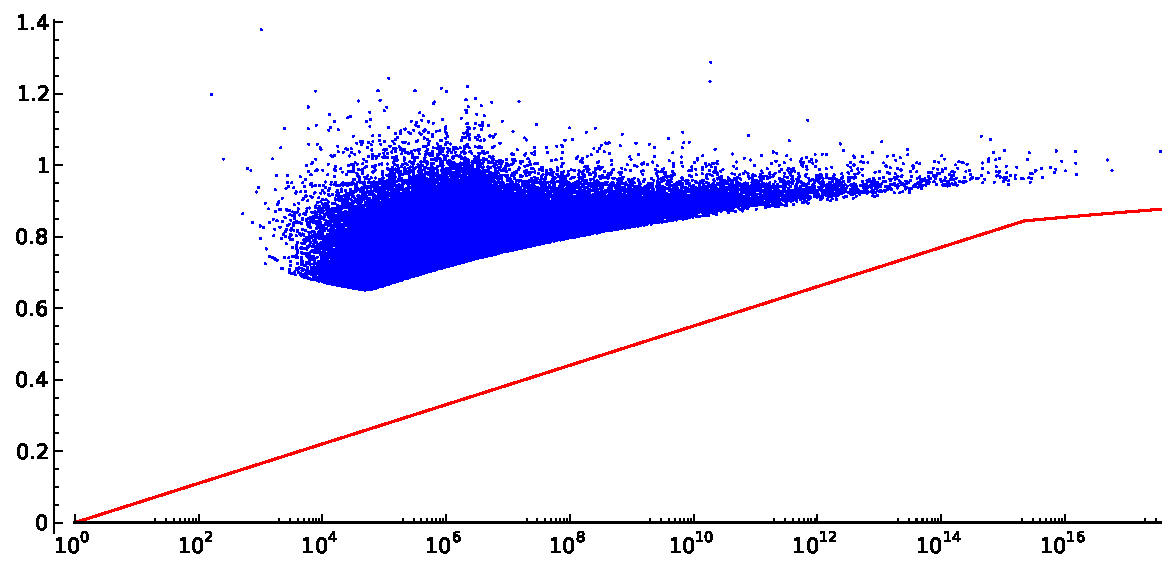
\includegraphics[width=\textwidth]{pics/c6_quality_plot.pdf}
    \caption{Quality as a function of $c_6$}
    \label{fig:abcdiscplot}
\end{figure}
\end{center}



Of course, due to Andrew Ohana's observations,
I have failed to convince you
that the strong ABC conjecture is actually true (see Section~\ref{sec:abchome}),
so I will understand if you do not consider this argument
to be convincing!

One goal of proving Theorem~\ref{thm:abcdisc} was to hopefully
give some explicit upper bound on the number of curves with
discriminant $|\Delta| < M$, assuming some effective version
of ABC, which might come out of the computations we've been
doing.   Of course, this is not what we get from our data...

See \cite[\S3.4]{bmsw:bulletins} for the following conjecture:
\begin{conjecture}
There are $cX^{5/6}$ curves with~$|\Delta|\le X$.
\end{conjecture}
\url{http://mathoverflow.net/questions/96285/average-rank-of-elliptic-curves-over-mathbbq}



The paper \cite{stein-watkins:ants5} is about systematic
enumeration of all pairs of integers $(c_4,c_6)$ such that
we have simultaneously
$$
|\Delta| \leq 10^{12} \quad\text{and}\quad
|c_4|\leq 1.44\cdot 10^{12}.
$$
We do not know that this gives us all curves with $|\Delta|\leq 10^{12}$,
but it does give us hundreds of millions of elliptic curves.
Here's a quick demo of using the Stein-Watkins tables from Sage
(see \url{http://wstein.org/ecdb/format.txt} for the meaning of the data).
\begin{lstlisting}
sage: v = SteinWatkinsPrimeData(0)
sage: c = v.next(); c
Stein-Watkins isogeny class of conductor 11
sage: list(c)
[[[0, -1, 1, 0, 0], '(1)', '1', '5'],
 [[0, -1, 1, -10, -20], '(5)', '1', '5'],
 [[0, -1, 1, -7820, -263580], '(1)', '1', '1']]
sage: v = SteinWatkinsPrimeData(1)
sage: c = v.next(); c
Stein-Watkins isogeny class of conductor 100000937
sage: list(c)
[[[1, 0, 1, -472, -3951], '[1]', '1', '1']]
sage: v = SteinWatkinsAllData(0)
sage: c = v.next(); c
Stein-Watkins isogeny class of conductor 11
sage: list(c)
[[[0, -1, 1, 0, 0], '(1)', '1', '5'],
 [[0, -1, 1, -10, -20], '(5)', '1', '5'],
 [[0, -1, 1, -7820, -263580], '(1)', '1', '1']]
sage: c = v.next(); c
Stein-Watkins isogeny class of conductor 14
sage: list(c)
[[[1, 0, 1, -1, 0], '(2,1)', '1', '6'],
 [[1, 0, 1, -11, 12], '[1,2]', '1', '6'],
 [[1, 0, 1, 4, -6], '(6,3)', '1', '6'],
 [[1, 0, 1, -36, -70], '[3,6]', '1', '6'],
 [[1, 0, 1, -171, -874], '(18,1)', '1', '2'],
 [[1, 0, 1, -2731, -55146], '[9,2]', '1', '2']]
sage: v = SteinWatkinsAllData(10)
sage: c = v.next(); c
Stein-Watkins isogeny class of conductor 1000002
sage: list(c)
[[[1, 1, 0, -63, -1539], '(3,6,1)', 'X', '1']]
\end{lstlisting}


\newpage
\section{The Conductor}
The conductor of an elliptic curve (defined over the rational numbers
or a number field) is another
invariant, like the minimal discrimant,
which encodes information about the local structure
of the elliptic curve at each bad prime.

\begin{theorem}
For each positive integer $N$,
there are finitely many elliptic curves over $\Q$
of conductor $N$, and there is an algorithm
to enumerate all of them that is polynomial
time in $N$.
\end{theorem}

\subsection{Reduction}
Suppose $E$ is an elliptic curve over $\Q$, and let
\begin{equation}\label{eq:condweq}
y^2 + a_1 xy + a_3 y = x^3 + a_2 x^2 + a_4 x + a_6
\end{equation}
be a global minimal model, so the $a_i$ are in $\Z$
and the discriminant $\Delta$ of the above equation is minimal
in absolute value, among all such Weierstrass equations for $E$.
For each prime number $p$, it makes sense to consider
the algebraic curve $E_{\F_p}$ over the finite field
$\F_p$ obtained by reducing \eqref{eq:condweq} modulo $p$.
The curve $E_{\F_p}$ is nonsingular if and only $p\nmid \Delta$.
When $p\mid \Delta$, there are three possible ways in which
$E_{\F_p}$ can be singular:
\begin{enumerate}
\item split nodal, e.g., $y^2=x^2(x+9)\pmod{11}$: there are two distinct
tangent lines at the singular point, with slopes in $\F_p$.
\item nonsplit nodal, e.g., $y^2=x^2(x+23) \pmod{37}$: there are two distinct tangent lines
at the singular point, but the slopes are in $\F_{p^2}$ instead
of $\F_p$.
\item cuspidal, e.g., $y^2=x^3\mod{17}$: there is a cuspidal singularity.
\end{enumerate}
We call the first two cases {\em multiplicative reduction}, since in those
cases the group of nonsingular points in $E_{\F_p}$ is $\G_m$ in
the split case, or it's the nontrivial twist of $\G_m$ in the nonsplit case.
We call the nodal case {\em additive reduction} since the group of nonsingular points is $\G_a$.  (To see these isomorphisms, draw a line through the singular point and consider the other point of intersection; this sets up a bijection between lines through the origin and nonsingular points.)

\subsection{``Definition'' via an incomplete formula that you will remember}
The conductor $N$ of $E$ is
$$
N = \prod_{p\mid\Delta} p^{v_p},
$$
where
$$
v_p = \begin{cases}
 1 & \text{ if $E$ has multiplicative reduction at $p$ } \\
 2 & \text{ if $E$ has additive reduction at $p\geq 5$ } \\
 \leq 5 & \text{ if $E$ has additive reduction at $p=3$ }\\
 \leq 8 & \text{ if $E$ has additive reduction at $p=2$ }.
 \end{cases}.
$$
In each additive case, $v_p\geq 2$.
The above is what everybody easily remembers about the conductor
of an elliptic curve.  I don't know of any simple
recipe for $v_p$ when $p=2,3$ is
a prime of additive reduction is complicated.

\begin{remark}
See Section~\ref{sec:condnf} below for a generalization (with
examples) of the above formula to number fields, where you will
find out whether
$v_\mathfrak{p}\leq 2$ for $\text{char}(\mathfrak{p})\geq 5$
and if $v_\mathfrak{p}$ can be arbitrarily large.
\end{remark}

The (partial) definition above is pretty arbitrary, lacking any
conceptual insight.   How does it generalize to elliptic curves
over numbers fields?  What does it have to do
with other things called ``conductors'' and ``levels''
in number theory?


\begin{quote}
{\bf Summary:} The conductor of $E$ is a product of the primes of bad
reduction for $E$.  It is exactly divisible by the primes of multiplicative
reduction, and divisible by $p^2$ for primes of additive reduction.
\end{quote}

\subsection{Definition using the functional equation}\label{sec:condfe}
Consider the $L$-series
$$
L(E,s) = \prod_{\text{all }p} \frac{1}{1-a_p p^{-s} + \eps(p)p^{1-2s}},
$$
where $\eps(p)=0$ if $p\mid \Delta$ and $\eps(p)=1$ otherwise, and
$$
 a_p = p + 1 - \# E_{\F_p}(\F_p).
$$
(NOTE: These $a_p$ have nothing to do with the coefficients
$a_i$ in the Weierstrass equation \eqref{eq:condweq} above.)
The deep theorem that every elliptic curve $E$ over $\Q$ is modular
implies that $L(E,s)$ extends (uniquely) to a holomorphic function
on the entire complex plane.  It's easier to understand the completed
$L$-series
$$
\Lambda(E,s) = 2\pi^{-s}\Gamma(s) L(E,s).
$$
The modularity theorem also implies that there is a unique integer
$N$ and sign $\epsilon\in \{1,-1\}$ such that $\Lambda(E,s)$ satisfies the following functional equation:
\begin{equation}\label{eqn:fe}
\Lambda(E,s) = \epsilon \cdot N^{1-s} \Lambda(E,2-s).
\end{equation}
The number $N$ is the {\em conductor of $E$}.



\begin{quote}
{\bf Summary:} The conductor of $E$ is a constant that appears
naturally in the functional equation for the $L$-series of $E$.
\end{quote}

\subsection{(*) Definition using modular forms}\label{sec:condmodform}
This section gets a star because it is how I think about
the conductor.


Expand the Euler product for
$L(E,s)$ from Section~\ref{sec:condfe}
to obtain a Dirichlet Series
$$
L(E,s) = \prod_{p} L_p(E,s) = \sum_{n\geq 1} \frac{a_n}{n^s},
$$
where the $a_n$ are integers.
The analytic function $L(E,s)$ on the complex plane is connected
via Mellin transform to the holomorphic function
$$
f_E(z) = \sum_{n\geq 1} a_n e^{2\pi i n z}
$$
on the upper half plane.  Alternatively, writing $q=q(z) = e^{2\pi i z}$,
we write
$$
f_E(q) = \sum_{n\geq 1} a_n q^n,
$$
which we view either as function of $z$ on the upper half plane,
or as a function of $q$ on the open unit disk.

The {\em conductor of $E$} is the smallest positive integer $N$
such that for all  matrices
$$
\gamma = \mtwo{a}{b}{c}{d} \in \Gamma_0(N)
  = \left\{\text{matrices in $\SL_2(\Z)$ that are upper triangular mod $N$}\right\},
$$
we have
$$f(\gamma(z))d(\gamma(z)) = f(z)dz,$$
where $\gamma(z) = \frac{az+b}{cz+d}$ is a linear fractional transformation.
Thus $f$ is a cuspidal modular form of level the conductor
$N$ of $E$.

\begin{quote}
{\bf Summary:} The conductor of $E$ is the level of the modular
form attached to $E$.
\end{quote}




\subsection{Definition using N\'eron models and Ogg's formula}

The {\em N\'eron model} $\cE$ of $E$ is the unique
smooth commutative group scheme over $\Z$ with
generic fiber $\cE_\Q = E$ such that for every smooth
scheme $X/\Z$ the natural map
$$
\cE(X) \to E(X_\Q)
$$
is an isomorphism.  The statement that the above
map is an isomorphism means that any morphism
$X_\Q \to E$ on generic fibers
can be extended uniquely to a morphism
$x \to \cE$ of schemes over $\Z$.
It is a theorem of N\'eron that his model exists.

The {\em component group} of $E$ at $p$ is the quotient
$$
 \Phi_{E,p} = \cE_{\F_p} / \cE_{\F_p}^0
$$
of the reduction of $\cE$ modulo $p$ by its identity component.
We have an exact sequence
$$
 0 \to \cE_{\F_p}^0 \to \cE_{\F_p} \to \Phi_{E,p} \to 0,
$$
and $\Phi_{E,p}$ is a finite flat group scheme over $\F_p$.

The exponent $v_p=\ord_p(N)$ in the conductor $N=\prod p^{v_p}$ is
$$
v_p = \ord_p(\Delta) - (\#\Phi_{E,p}(\Fbar_p) - 1) \qquad\text{(Ogg's formula)},
$$
where $\Delta$ is the minimal discriminant of $E$.

Software such as Sage uses Tate's algorithm to compute
$\#\Phi_{E,p}(\Fpbar)$.  This is implemented in Sage over
arbitrary number fields.

Ogg's formula implies that given an elliptic curve $E$,
knowing any two of the following invariants determines the third:
\begin{enumerate}
\item\label{condinv:1} The minimal discriminant of $E$.
\item\label{condinv:2}  The conductor of $E$.
\item\label{condinv:3}  The orders of the components groups of $E$.
\end{enumerate}
For example, Aly Deines uses this in her thesis work (extending
work of Shuzo Takahashi and Ken Ribet),
where she uses Shimura curves to determine invariants
\ref{condinv:2} and \label{condinv:3} of a certain curve,
which then determines \ref{condinv:2}.
She then studies hypothesis under which 1 and
2 determine the curve itself.

The Tamagawa numbers $c_p$ of  $E$ are
$$
c_p = \#\Phi_{E,p}(\F_p).
$$
Since $\Phi_{E,p}(\F_p)$ is a subgroup of $\Phi_{E,p}(\Fbar_p)$,
the numbers $c_p$ divide the numbers
$\overline{c}_p = \#\Phi_{E,p}(\Fbar_p)$
in Ogg's formula.
The Tamagawa numbers appear in the {\em conjectural} formula of Birch
and Swinnerton-Dyer:
$$
\frac{L^{r}(E,1)}{r!} =
  \frac{\Omega_E \cdot \prod_{p\mid N} c_p \cdot \Reg_E \cdot \#\Sha(E)}
       {\#E(\Q)_{\tor}^2},
$$
where $r$ is conjectured to be both $\ord_{s=1}L(E,s)$
and the rank of $E(\Q)$.


\begin{quote}
{\bf Summary:} The conductor of an elliptic curve is obtained
from the minimal discriminant by reducing the power of each
prime by the order of the corresponding component group (minus 1).
\end{quote}



\subsection{Definition using Galois representations}
Let $E$ be any elliptic curve over $\Q$.
For each prime $\ell$, consider the two-dimensional
Galois representation
$$
 \rhobar_{E,\ell}:G_\Q \to \Aut(E[\ell])
$$
obtained by considering the action of the
absolute Galois group $G_\Q=\Gal(\Qbar/\Q)$
on the group
$$
E[\ell] = \{P \in E(\Qbar) : \ell P = 0\}
$$
of $\ell$-torsion points on $E$.
We associate an integer $N(\rhobar_{E,\ell})$, called
the {\em Serre level}, to
this representation. Note that Serre level, as we will define it, makes sense for {\em any}
Galois representation
$\rhobar:G_{\Q} \to V$
over $\F_\ell$,
not just for representations
attached to elliptic curves.
Write
$$
 N(\rhobar) = \prod_{\text{primes $p\neq \ell$}} p^{n(p)},
$$
where it remains to define the numbers $n(p)$, which will measure
subtle properities of the ramification of $\rhobar$.

Since $\rhobar$ is continuous and $\Aut(V)$ is a finite set,
there is a finite Galois exension $K/\Q$ such that $\rhobar$
factors through $\Gal(K/\Q)$.  We have a surjective
map $G_{\Q} \onto \Gal(K/\Q)$ followed by an inclusion
$\Gal(K/\Q)\subset \Aut(V)$, with $K$ a Galois extension.
More concreately, the field $K$ is
the extension of $\Q$ generated by the $x$ and $y$ coordinates
of all $\ell$-torsion points on $E$, which we often write
$$
  K = \Q(E[\ell]).
$$

Fix a prime number $p$, let $\O_K$ be the ring of integers
of $K$,, then factor $p$ as a product of prime ideals
$$
  p\O_K = \prod_{i=1}^g \fp_i.
$$
Let $\fp$ be a choice of any one of the $\fp_i$; which
we choose does not impact the definition at all, as it turns out, since
the primes $\fp_i$ are all conjugate under the action of
$\Gal(K/\Q)$.
With these choices, the decomposition group is
$$
  D = \{\sigma \in \Gal(K/\Q) : \sigma(\fp) = \fp\}.
$$
Consider the finite field $\F_\fp = \O_K/\fp$.
One proves that there is an exact sequence
$$
  1 \to I \to D \to \Gal(\F_\fp / \F_p) \to 1,
$$
where the {\em inertia group} $I$ is by definition the kernel,
and surjectivity of the map $D \to \Gal(\F_\fp / \F_p)$
is not supposed to be obvious.
and surjectivity of the map $D \to \Gal(\F_\fp / \F_p)$
is not supposed to be obvious.
Thus
$$
  I = \{\sigma \in D : \sigma(x) \equiv x \pmod{\fp} \text{ all } x \in \O_K\},
$$
and it is natural to define further smaller subgroups of $D$ by letting
\begin{align*}
  G_i &= \{\sigma \in I : \sigma(x) \equiv x \pmod{\fp^{i+1}} \text{ all } x \in \O_K \}\\
      &= \ker(I \to \Aut((\O_K/\fp^{i+1}) / (\Z/p^{i+1}\Z)))
\end{align*}
for all $i\geq 0$.  These finite groups
$$G_0 \supseteq G_1 \supseteq G_2 \supseteq \cdots $$
are the {\em higher ramification groups} associated
to our fixed choice of prime $\fp$ over~$p$.

Finally, we define
$$
n(p) = \sum_{i=0}^{\infty} \frac{1}{[G_0:G_i]}\dim V/V^{G_i},
$$
where
$$
  V^{G_i} = \{x \in V : \sigma(x) = x \text{ all } \sigma\in G_i\}.
$$
The groups $G_i$ are trivial for all sufficiently large $i$,
so the sum has only finitely many nonzero terms.
The representation sentation $V$ is unramified at $p$ if and only
if $G_0$ acts trivially, so we have $n(p)=0$  if and only
if $V$ is unramified at $p$ (for primes $p\neq \ell$).

Returning to our elliptic curve $E$, we have now defined,
for each prime $\ell$, an integer
$N(\rhobar_{E,\ell})$, which is by definition coprime to $\ell$.
\begin{definition}[Conductor]
The {\em conductor} $N_E$ of $E$ is the least common multiple  of
the integers $N(\rhobar_{E,\ell})$, over all primes $\ell$.
\end{definition}

\begin{corollary}
A prime $p$ is ramified in $\Q(E[\ell])$ for some $\ell\neq p$
if and only if $p\mid N_E$.
\end{corollary}

The {\em criterion of N\'eron-Ogg-Shafarevich} is an improvement
of the above corollary---it's a criterion purely
in terms of ramification---for whether or not a prime
$p$ is a prime of bad reduction for an elliptic curve.
\begin{theorem}[Criteron of N\'eron-Ogg-Shafarevich]
A prime $p$ is ramified in $\Q(E[\ell])$ for all but
finitely many $\ell\neq p$ if and only if $p\mid N_E$.
\end{theorem}
(In fact, their theorem is stronger, asserting that $p\mid N_E$
if and only if $p$ is ramified in $\Q(E[\ell^\infty])$ for
all $p\neq \ell$.)


\subsubsection{Serre's Conjecture}
Since we're so close, it's worth mentioning Serre's conjecture,
though we have not yet discussed how to
associate Galois representations $\rhobar_{f,\lambda}$
to modular forms~$f$.
\begin{theorem}[Serre's Conjecture]
Suppose $\rhobar:G_{\Q}\to V$
is a 2-dimensional absolutely irreducible
mod~$\ell$ Galois representation such that
$$\det(\rhobar(\text{\rm complex conjugation})) =-1.$$
Then there is a modular eigenform of level
$N(\rhobar)$ such that $\rhobar \ncisom \rhobar_{f,\lambda}$,
for some prime $\lambda\mid \ell$.
\end{theorem}
Serre also gives a formula for a weight $k(\rhobar)\in\Z$, and
conjectures that $f\in S_{k(\rhobar)}(\Gamma_1(N(\rhobar)))$.
I {\em think} all cases of Serre's conjectures are now known
(unless there's some weird corner case when $\ell=2$), due to
work of Khare, Wintenberger, Dieulefait, Ribet, Diamond, and many
others, which grew out of Taylor-Wiles's work on Fermat's Last Theorem.
There are also generalizations of this result to totally real
fields.  Computational, the above theorem is often extremely
helpful, since it provides a specific finite dimensional space
in which the relevant modular form must live.


\begin{quote}
{\bf Summary:} The conductor of an elliptic curve is the least common multiple
of the Serre levels of the mod $\ell$ Galois representations associated to the
elliptic curve.
\end{quote}

% Yannick
\subsection{The conductor of E over a number field}\label{sec:condnf}

Then
$$
N = \prod_{\mathfrak{p}} \mathfrak{p}^{f(E/K_{\mathfrak{p}})}
$$
where the product runs over all nonzero prime ideals $\mathfrak{p}$
of $\O_K$ and
$$
f(E/K_\mathfrak{p}) = \left\{\begin{array}{ll}
0 & \text{if $E/K_{\mathfrak{p}}$ has good reduction at $\mathfrak{p}$} \\
1 & \text{if $E/K_{\mathfrak{p}}$ has multiplicative
reduction at $\mathfrak{p}$} \\
2 & \text{if $\mathfrak{p}|p \geq 5$ and $E/K_{\mathfrak{p}}$
has additive reduction at $\mathfrak{p}$} \\
\end{array}\right.
$$
and
$$
2 \leq f(E/K_{\mathfrak{p}}) \leq 2 + 3 \, \mathrm{ord}_{\mathfrak{p}}(3)
 + 6 \, \mathrm{ord}_{\mathfrak{p}}(2)
$$
if $\mathfrak{p}|p$ for $p \in \{2, 3\}$ and $E/K_{\mathfrak{p}}$ has
additive reduction at $\mathfrak{p}$ (note that only one of
$\mathrm{ord}_{\mathfrak{p}}(3)$ and $\mathrm{ord}_{\mathfrak{p}}(2)$ is
nonzero).

\begin{lstlisting}
sage: E = EllipticCurve('256a')
sage: print E
sage: for n in range(1,8):
sage:     K.<alpha> = NumberField(x^n - 2)
sage:     EK = E.base_extend(K);
sage:     print n, EK.conductor().factor()
Elliptic Curve defined by y^2 = x^3 + x^2 - 3*x + 1 over Rational Field
(Fractional ideal (2))^8
(Fractional ideal (alpha))^10
(Fractional ideal (alpha))^20
(Fractional ideal (alpha))^8
(Fractional ideal (-alpha))^32
(Fractional ideal (2, alpha))^26
(Fractional ideal (2, alpha))^44
\end{lstlisting}

\begin{lstlisting}
sage: E = EllipticCurve('243a');
sage: print E
sage: for n in range(1,8):
sage:     K.<alpha> = NumberField(x^n - 3)
sage:     EK = E.base_extend(K);
sage:     print EK.conductor().factor()
Elliptic Curve defined by y^2 + y = x^3 - 1 over Rational Field
(Fractional ideal (3))^5
(Fractional ideal (alpha))^8
(Fractional ideal (alpha))^3
(Fractional ideal (alpha))^14
(Fractional ideal (-alpha))^17
(Fractional ideal (3, alpha))^4
(Fractional ideal (3, alpha))^23
\end{lstlisting}

\section{Modularity of elliptic curves over $\Q$}
Barry Mazur once wrote a great article entitled {\em Number Theory as Gadfly}
which is about what it means for an elliptic curve
over $\Q$ to be {\em modular}.

\begin{theorem}[Breuil, Conrad, Diamond, Taylor, Wiles]\label{thm:modularity}
Every elliptic curve over $\Q$ is modular.
\end{theorem}
This theorem is incredibly
important to numerous algorithms for computing with elliptic curves.
As with the definition of conductor, there
are many
ways of viewing modularity, with deep connections between them.

\subsection{Definition using modular forms}

Let $E$ be an elliptic curve.
In Section~\ref{sec:condmodform} we defined a function
$$
f = f_E(q) = \sum_{n=1}^{\infty} a_n q^n,
$$
and it is relatively easy to prove that $f_E$ defines
a holomorphic function on the upper half plane
$$
  \h = \{z \in \C : \Im(z) > 0\} \subset \C.
$$
We then defined the conductor $N$ as the smallest positive
integer so that
$$f(z)dz = \frac{f(q)}{q} dq$$
is invariant
under the action of the congruence subgroup
$\Gamma_0(N)$.   Theorem~\ref{thm:modularity} is  the assertion
that there is {\em some} $N$ such that $f$ is invariant under $\Gamma_0(N)$.
The function~$f$ is then a normalized cuspidal
modular eigenforms level $N$ and weight $2$, and we write
$$
 f \in S_2(\Gamma_0(N))_{\new}
$$




\begin{quote}
{\bf Summary:} An elliptic curve $E$ over $\Q$ is modular if
the function $f(q) = \sum a_n q^n$, with $a_p = p+1-\#E(\F_p)$
is a modular form.
\end{quote}

\subsection{(*) Definition using systems of Hecke eigenvalues}\label{sec:modhecke}
This section gets a star because it is how I think about
modularity.

The {\em Hecke algebra} is a commutative ring $\T$ that acts on
the space $S_2(\Gamma_0(N))$ of cusp forms. The Hecke algebra
is generated by Hecke operators $T_n$, one for each integer $n$
$$
  \T = \Z[T_1, T_2, T_3, \ldots].
$$
That $f=\sum a_n q^n$ is a normalized eigenform means that  for each
integer $n$, we have
$$
  T_n(f) = a_n \cdot f,
$$
i.e., the coefficients of $f$ are the eigenvalues of the linear
transformations $T_n$.  There are also recurrences satisfied
by the $T_n$, so that knowing them for prime $n$ determines
all of them.
Thus alternatively, $E$ is modular if there is some eigenvector
$v \in S_2(\Gamma_0(N))$ such that for all primes $p$ we have
$$
  T_p(v) = (p+1 - \# E(\F_p)) \cdot v.
$$

\begin{quote}
{\bf Summary:} An elliptic curve $E$ over $\Q$ is modular if
the point counts $\# E(\F_p)$ are encoded in the system
of Hecke eigenvalues of some eigenvector in $S_2(\Gamma_0(N))$.
\end{quote}

  Moreover, and this is key, one can replace $S_2(\Gamma_0(N))$ by any $\T$-module that is isomorphic
to it.


\subsection{Definition in terms of modular curves}

Let $E$ be an elliptic curve over $\Q$, let $N$
be the conductor of $E$, and consider the left action
of $\Gamma_0(N)$ on the extended upper half plane
$$
\h^*=\h\cup\Q\cup\{i\infty\}
$$
by linear fractional transformations:
$$
\mtwo{a}{b}{c}{d}(z) = \frac{az+b}{cz+d}.
$$
The modular curve of level $\Gamma_0(N)$ is the compact Riemann {\em surface}
$$
  X_0(N)(\C) = \Gamma_0(N) \backslash \h^*.
$$


For example, when $N=11$, the real surface $X_0(11)(\C)$ has genus 1:
\begin{lstlisting}
sage: dimension_cusp_forms(11)
1
sage: u = var('u')
sage: revolution_plot3d((cos(u),sin(u)),(u,0,2*pi),axis=(2,0),color='green',
      opacity=.7, mesh=True, frame=False)
\end{lstlisting}
\begin{center}
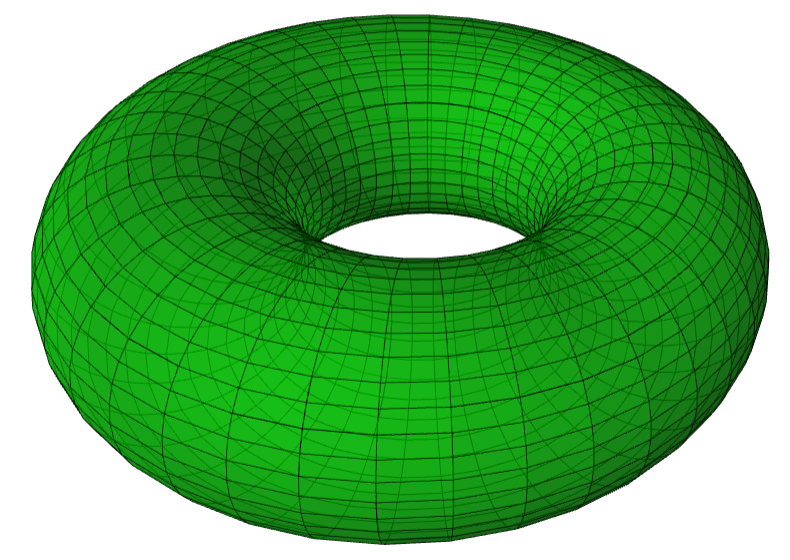
\includegraphics[width=.7\textwidth]{pics/torus}
\end{center}


Developing the theory of modular functions, one proves that
$X_0(N)(\C)$ is the set of complex points of an algebraic curve
$X_0(N)$ defined over $\Q$ (or even over $\Z$ -- see Katz-Mazur!).
Theorem~\ref{thm:modularity} then asserts that there is a surjective
morphism of algebraic curves $X_0(N)\to E$.

\begin{remark}
Fun and useless fact:
There are modular curves $X_0(N)$ of genus $g$ for each $g\leq 149$,
but there is no modular curve of genus $150$.  See Csirik, et al.
\end{remark}

\subsection{Definition in terms of $L$-series}

In Section~\ref{sec:condfe} we defined the conductor of $E$
as a constant that arises in the functional equation
for $L(E,s)$.   The assertion that $E$ is modular is
{\em a priori} a {\em stronger} statement than the assertion
that $L(E,s)$ is entire and satisfies the functional
equation \eqref{eqn:fe}.  If $E$ is modular, than $L(E,s)=L(f,s)$
is indeed entire and satisfies the functional equation;
however, as $f$ is a modular form, we also have for
every Dirichlet character $\chi$,  that
$L(f^{\chi},s)$ is also entire and satisfies a functional
equation.  There is a {\em converse theorem}, due to Weil,
which asserts that if $L(E,s)$ is entire and satisfies
a functional equation, {\em and} so do ``all of its twists'', then
$L(E,s)=L(f,s)$ for some modular form $f$.
{\em Warning: I don't know the precise formulation
of this statement -- exercise for a student in class to fill
this in.}

The above converse theorem was considered for a long time to be
the best evidence for the modularity conjecture before
it was proved.  This might be why the modularity statement
has had (at least) the following names:
\begin{enumerate}
\item The conjecture of Weil
\item The Taniyama-Shimura-Weil conjecture
\item The Taniyama-Weil conjecture:\\ page 341 of {\em A Course in Number Theory}, By H. E. Rose
\item The Shimura-Taniyama conjecture:\\ \url{http://www.ams.org/notices/199511/forum.pdf}
\item The Modularity theorem:\\ \url{http://en.wikipedia.org/wiki/Modularity_theorem}
\end{enumerate}

\section{Converse theorems}


\section{Modularity over real quadratic fields}

The following huge result appeared on the arxiv a few days ago (see
\url{http://arxiv.org/abs/1310.7088}).
\begin{theorem}[Freitas, Le Hung, Siksek]
Every elliptic curve over a real quadratic field is modular.
\end{theorem}
Part of their motivation was FLT over real quadratic fields, which
is the subject of another paper they just posted at \url{http://arxiv.org/abs/1307.3162}.


\subsection{Definition in terms of Hilbert modular forms}

We sketch what it means for an elliptic curve $E$
over a real quadratic field $K=\Q(\sqrt{d})$ to be
{\em modular}.

Let $\n$ be an ideal in the ring $\O_K$ of integers of $K$,
and fix two embeddings $\iota_1:K\hookrightarrow \R$
and $\iota_2:K\hookrightarrow\R$.
Let $\GL_2^+(\O_K)$ be the group of $2\times 2$ matrices
$\gamma$ with entries in $\O_K$ such that
both $\iota_1(\det(\gamma))>0$ and
$\iota_2(\det(\gamma))>0$.
The analogue over $K$ of the congruence subgroup $\Gamma_0(N)\subset\SL_2(\Z)$ is
$$
\Gamma_0(\n)
 = \left\{
\mtwo{a}{b}{c}{d} \in \GL_2^+(\O_K)  :
  c \in \n
   \right\}.
$$
For $\gamma=\mtwo{a}{b}{c}{d}\in \Gamma_0(\n)$,
we let $a_i,b_i,c_i,d_i\in\R$ denote the entries
of $\iota_i(\gamma)$, for $i=1,2$.

A {\em holomorphic function} on
an open subset of $\C\times \C$ is a complex-valued function
that is continuous and holomorphic in each of its variables.
A {\em Hilbert modular form} over $K$ of parallel weight $(2,2)$
and level $\n$
is a holomorphic function
$$
f = f(z_1,z_2):\h\times \h \to \C
$$
on the product of two copies of the upper half plane such that
for all $\gamma \in \Gamma_0(\n)$, we have
$$
  f(\gamma_1(z_1), \gamma_2(z_2))
     = \frac{(c_1 z_1 + d_1)^2}{\det \gamma_1}
       \cdot  \frac{(c_2 z_2 + d_2)^2}{\det \gamma_2}
       \cdot f(z_1, z_2).
$$
Let $M_{(2,2)}(\Gamma_0(\n))$ denote the space of Hilbert modular forms,
as above.

For simplicity, assume that $K$ has narrow class number $1$.
As in Section~\ref{sec:modhecke}, there are commuting Hecke operators
$\T_\fp$ acting on $M_{(2,2)}(\Gamma_0(\n))$,
for each nonzero prime ideal $\fp$ of $\O_K$.
The elliptic curve $E$ over $K$ is {\em modular} if there
is an eigenvector $f \in M_{(2,2)}(\Gamma_0(\n))$ such that
for all $\fp$ we have
$$
  T_\fp(f) = (\text{Norm}(\fp) + 1 - \#E(\F_\fp)) \cdot f.
$$





\section{Computing all elliptic curves over the rational numbers using modular symbols}

Cremona's book {\em Algorithms for Modular Elliptic Curves} is about the following:

\begin{quote}
\noindent{\bf Problem: }
Given an integer $N$, find all elliptic curves over $\Q$
of conductor $N$.
\end{quote}

Recall from Section~\ref{sec:modhecke} that for an elliptic
curve $E$ to be modular means that the integers
$$
  a_p = a_p(E) = p + 1 - \#E(\F_p) \in \Z,
$$
for $p$ prime, are also the eigenvalues of the
Hecke operators $T_p$ acting on some eigenvector
in the space of cusp forms $S_2(\Gamma_0(N))$.

To solve the above problem, we have the following
strategy:
\begin{enumerate}
\item Compute a $\T$-module $V$ such that for every
elliptic curve of conductor $N$, the system of
eigenvalues $\{a_p(E)\}$ is guaranteed to occur in $V$.
For example, one could take $V=S_2(\Gamma_0(N))$.
\item Given finitely many of the integers $\{a_p(E)\}$,
find an equation for a curve $E$ with those $a_p$.
\item Find the finitely many curves isogenous to $E$.
\end{enumerate}

\subsection{Computing systems of eigenvalues}
Modular symbols is one
powerful systematic approach to finding all systems
of rational Hecke eigenvalues $a_p(E)$ corresponding
to elliptic curves of conductor $N$.
The basic idea is to explicitly compute the homology group
$$
  H_1(X_0(N),\Q),
$$
which is equipped with an action of Hecke operators $T_p$.
Then we do linear algebra with these matrices
to compute the systems of Hecke eigenvalues.

Recall that $X_0(N)=\Gamma_0(N)\backslash \h\cup \{\Q\}\cup\{\infty\}$,
where the {\em cusps} are the elements of
$$
\P^1(\Q) = \{\Q\}\cup\{\infty\}.
$$
To compute $H_1(X_0(N),\Q)$, we consider the slightly
bigger relative homology group
$$
H_1(X_0(N),\Q) \subset H_1(X_0(N),\Q; \{\text{cusps}\}).
$$
One can prove that $H_1(X_0(N),\Q; \{\text{cusps}\})$ is
generated by all geodesic paths $\{\alpha,\beta\}$
between elements $\alpha,\beta \in \P^1(\Q)$.  Note that
the notation $\{\alpha,\beta\}$ means the path {\em from}
$\alpha$ to $\beta$, i.e., it is {\em ordered}, despite looking
like a set -- this is a historical accident, I guess.

\subsubsection{Manin's trick}
Manin observed using continued fractions that
there is an explicit
finite subset of paths $\{\alpha,\beta\}$
that generate $H_1(X_0(N),\Q; \{\text{cusps}\})$.


\subsection{Computing a curve $E$ with given $a_p$}

\subsection{Finding all curves isogenous to $E$}


\section{Compute all elliptic curves over real quadratic fields using quaternion algebras}

\section{Integral points and discriminant equations}



\chapter{Prime Numbers}

Main unsolved problem: the Riemann Hypothesis



\section{Infinitely many primes}
\section{The Prime number theorem}
\section{The Riemann hypothesis}
\section{The Explicit Formula}
\section{Generalizations to number fields}


\chapter{Arithmetic of Number Fields}
Main unsolved problem: class number 1 fields

\section{Class groups}
\section{The Gauss class number problem}
\section{Number fields of class number 1}
 (Cohen-lenstra, Bharghava)



\chapter{Diophantine Equations: Fermat and ABC}
Main unsolved problem: ABC conjecture

\section{Fermat's Last Theorem}
\section{The ABC Conjecture}
\section{Generalized Fermat equations}



\chapter{Elliptic Curves}
Important unsolved problem: the BSD conjecture (computing Mordell-Weil groups)

\section{The Group law}
\section{The Mordell-Weil theorem}
\section{Mazur's classification of torsion subroups}
\section{The $L$-series}
analytic continuation and functional equation (modularity)
\section{The Birch and Swinnerton-Dyer conjecture}
\section{The Hasse bound}
\section{The Explicit Formula}



\chapter{Modular Forms}
Important unsolved problem: modularity of elliptic curves
over totally real fields

\section{Ramanujan bound}
\section{Galois representations attached to modular forms}
\section{Modularity of elliptic curves}




\chapter{Public-key Cryptography}

Important unsolved problem: how difficult is the discrete log problem?

\section{Protocols: Diffie-Hellman, RSA, ElGamal, ...}
\section{Discrete log problem (baby-step, giant-step)}


\bibliographystyle{amsalpha}
\bibliography{biblio}

\end{document}

%sagemathcloud={"zoom_width":150}
